% Options for packages loaded elsewhere
\PassOptionsToPackage{unicode}{hyperref}
\PassOptionsToPackage{hyphens}{url}
%
\documentclass[
]{book}
\usepackage{amsmath,amssymb}
\usepackage{iftex}
\ifPDFTeX
  \usepackage[T1]{fontenc}
  \usepackage[utf8]{inputenc}
  \usepackage{textcomp} % provide euro and other symbols
\else % if luatex or xetex
  \usepackage{unicode-math} % this also loads fontspec
  \defaultfontfeatures{Scale=MatchLowercase}
  \defaultfontfeatures[\rmfamily]{Ligatures=TeX,Scale=1}
\fi
\usepackage{lmodern}
\ifPDFTeX\else
  % xetex/luatex font selection
\fi
% Use upquote if available, for straight quotes in verbatim environments
\IfFileExists{upquote.sty}{\usepackage{upquote}}{}
\IfFileExists{microtype.sty}{% use microtype if available
  \usepackage[]{microtype}
  \UseMicrotypeSet[protrusion]{basicmath} % disable protrusion for tt fonts
}{}
\makeatletter
\@ifundefined{KOMAClassName}{% if non-KOMA class
  \IfFileExists{parskip.sty}{%
    \usepackage{parskip}
  }{% else
    \setlength{\parindent}{0pt}
    \setlength{\parskip}{6pt plus 2pt minus 1pt}}
}{% if KOMA class
  \KOMAoptions{parskip=half}}
\makeatother
\usepackage{xcolor}
\usepackage{longtable,booktabs,array}
\usepackage{calc} % for calculating minipage widths
% Correct order of tables after \paragraph or \subparagraph
\usepackage{etoolbox}
\makeatletter
\patchcmd\longtable{\par}{\if@noskipsec\mbox{}\fi\par}{}{}
\makeatother
% Allow footnotes in longtable head/foot
\IfFileExists{footnotehyper.sty}{\usepackage{footnotehyper}}{\usepackage{footnote}}
\makesavenoteenv{longtable}
\usepackage{graphicx}
\makeatletter
\def\maxwidth{\ifdim\Gin@nat@width>\linewidth\linewidth\else\Gin@nat@width\fi}
\def\maxheight{\ifdim\Gin@nat@height>\textheight\textheight\else\Gin@nat@height\fi}
\makeatother
% Scale images if necessary, so that they will not overflow the page
% margins by default, and it is still possible to overwrite the defaults
% using explicit options in \includegraphics[width, height, ...]{}
\setkeys{Gin}{width=\maxwidth,height=\maxheight,keepaspectratio}
% Set default figure placement to htbp
\makeatletter
\def\fps@figure{htbp}
\makeatother
\setlength{\emergencystretch}{3em} % prevent overfull lines
\providecommand{\tightlist}{%
  \setlength{\itemsep}{0pt}\setlength{\parskip}{0pt}}
\setcounter{secnumdepth}{5}
\usepackage{booktabs}
\ifLuaTeX
  \usepackage{selnolig}  % disable illegal ligatures
\fi
\usepackage[]{natbib}
\bibliographystyle{plainnat}
\usepackage{bookmark}
\IfFileExists{xurl.sty}{\usepackage{xurl}}{} % add URL line breaks if available
\urlstyle{same}
\hypersetup{
  pdftitle={Maple},
  pdfauthor={Ashan J},
  hidelinks,
  pdfcreator={LaTeX via pandoc}}

\title{Maple}
\author{Ashan J}
\date{2024-10-27}

\usepackage{amsthm}
\newtheorem{theorem}{Theorem}[chapter]
\newtheorem{lemma}{Lemma}[chapter]
\newtheorem{corollary}{Corollary}[chapter]
\newtheorem{proposition}{Proposition}[chapter]
\newtheorem{conjecture}{Conjecture}[chapter]
\theoremstyle{definition}
\newtheorem{definition}{Definition}[chapter]
\theoremstyle{definition}
\newtheorem{example}{Example}[chapter]
\theoremstyle{definition}
\newtheorem{exercise}{Exercise}[chapter]
\theoremstyle{definition}
\newtheorem{hypothesis}{Hypothesis}[chapter]
\theoremstyle{remark}
\newtheorem*{remark}{Remark}
\newtheorem*{solution}{Solution}
\begin{document}
\maketitle

{
\setcounter{tocdepth}{1}
\tableofcontents
}
\chapter{Introduction to Maple}\label{introduction-to-maple}

This is temporary file

\section{What is Maple?}\label{what-is-maple}

\begin{itemize}
\tightlist
\item
  Maple is a Symbolic Computation System or Computer Algebra System which can be used to obtain exact analytical solutions to many mathematical problems, including integrals, systems of equations, differential equations, and problems in linear algebra.
\item
  It also has the capability of plotting functions in 2D and 3D and displaying animations.
\item
  Maple can perform calculations in binding speed, but one has to be responsible for making these calculations meaningfully and mathematically correct.
\end{itemize}

\section{Using a Maple Worksheet}\label{using-a-maple-worksheet}

The following figure shows the Maple window with a blank Maple worksheet and this window contains:

\begin{itemize}
\tightlist
\item
  a menu bar across the top with menus:
\item
  a tool bar immediately below the menu bar, with button-based short cuts to common operations;
\item
  a context bar directly below the tool bar, with controls specific to the task being performed;
\end{itemize}

\begin{figure}
\centering
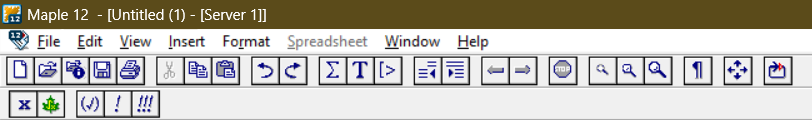
\includegraphics{figures/Lesson 1/fig1.png}
\caption{The menu bar, tool bar, and context bar.}
\end{figure}

\begin{itemize}
\tightlist
\item
  a window, containing a Maple prompt {[}\textgreater, called a worksheet;
\item
  a status bar at the bottom, with boxes marked Ready, Time and Memory
\end{itemize}

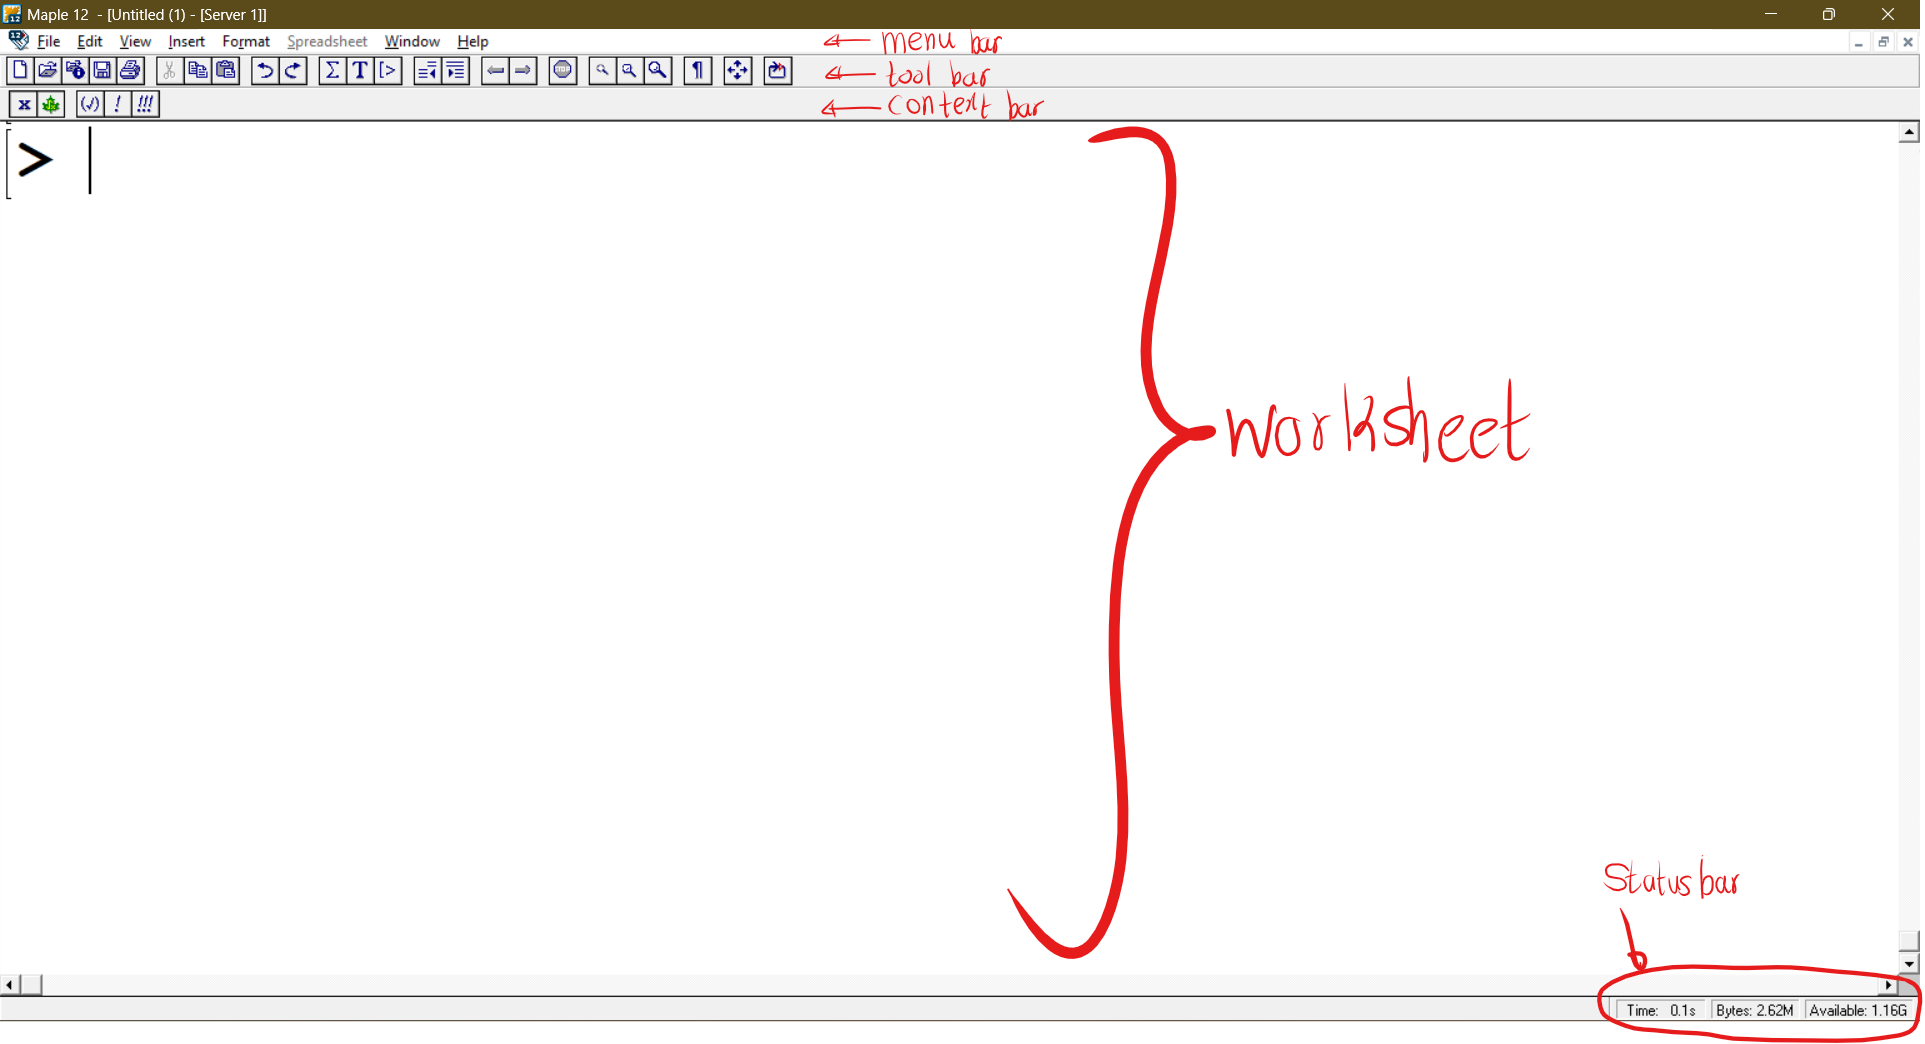
\includegraphics{figures/Lesson 1/fig2.png}

From the File menu, select the options \textbf{Save} or \textbf{Save As} to save the active Maple classic worksheet.
Maple classic worksheets are saved with the extension ``.mws'', but in the standard interface, Maple worksheets are saved with the extension ``.mw''

\section{Entering Maple Commands}\label{entering-maple-commands}

\begin{itemize}
\tightlist
\item
  The `` \textgreater{} '' is the command prompt in Maple. That is where you type your commands or statements.
\item
  Every command in Maple should end with a semicolon(;) or a colon(:).\\
  (If you use a semicolon then the result of the command will be displayed. If you use a colon then the result will not be displayed.)
  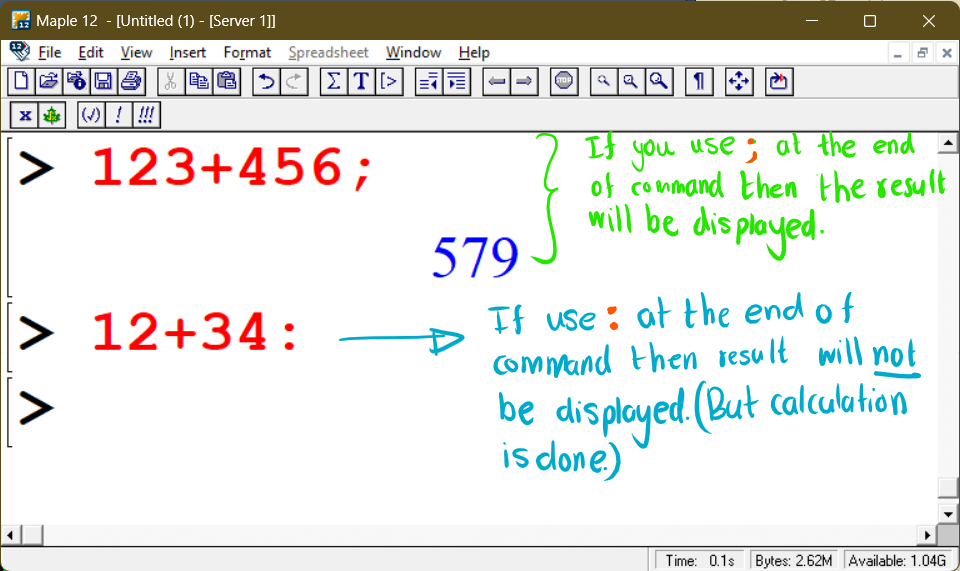
\includegraphics{figures/Lesson 1/fig3.png}
\item
  If you want to make any comments you can use the text format by clicking on the box \texttt{T} in the tool bar or use the symbol \texttt{\#}.
\end{itemize}

\section{Arithmetic operations}\label{arithmetic-operations}

Arithmetic operators follow the same precedence rules as in Mathematics, and these are brackets, of, division, multiplication, addition and subtraction (BODMAS). Usual arithmetic operations can perform easily with Maple.

\begin{verbatim}
[> 312+121;
\end{verbatim}

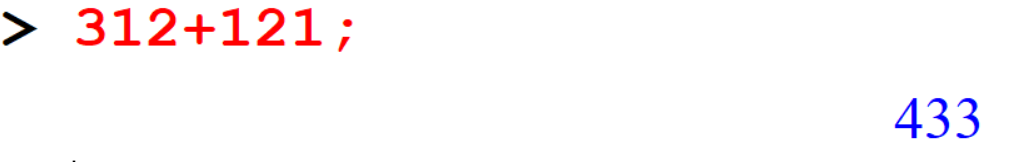
\includegraphics{figures/Lesson 1/fig4.png}

\begin{verbatim}
> 125-45;
\end{verbatim}

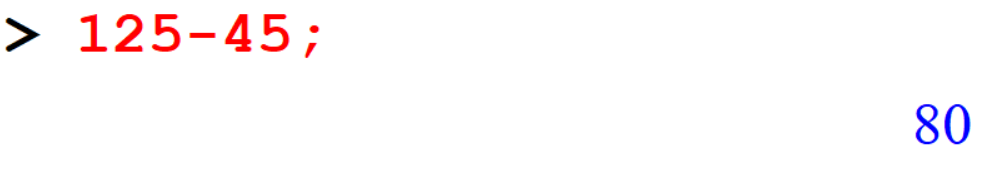
\includegraphics{figures/Lesson 1/fig5.png}

The \texttt{*} key is used for multiplication, \texttt{/} for division and \texttt{\^{}} for the power.

\begin{verbatim}
[> 13*267;
\end{verbatim}

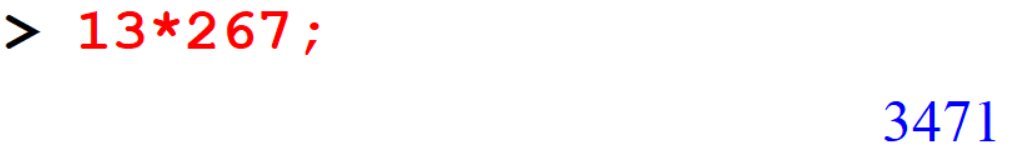
\includegraphics{figures/Lesson 1/fig6.png}

\begin{verbatim}
[> 565/5;
\end{verbatim}

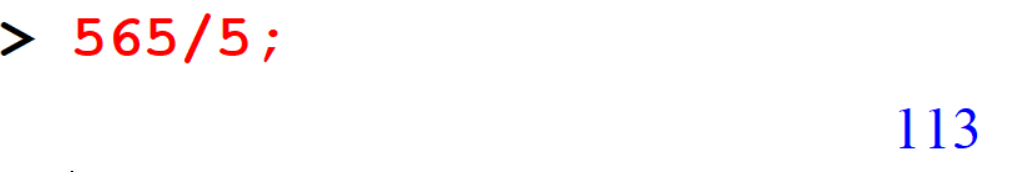
\includegraphics{figures/Lesson 1/fig7.png}

\begin{verbatim}
[> 561/5;
\end{verbatim}

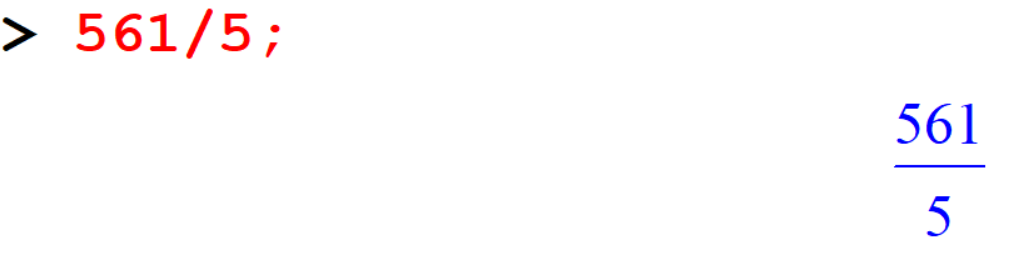
\includegraphics{figures/Lesson 1/fig8.png}

\begin{verbatim}
[> 125-45; 13*267; 12345/5; #Three arithmetic operations
\end{verbatim}

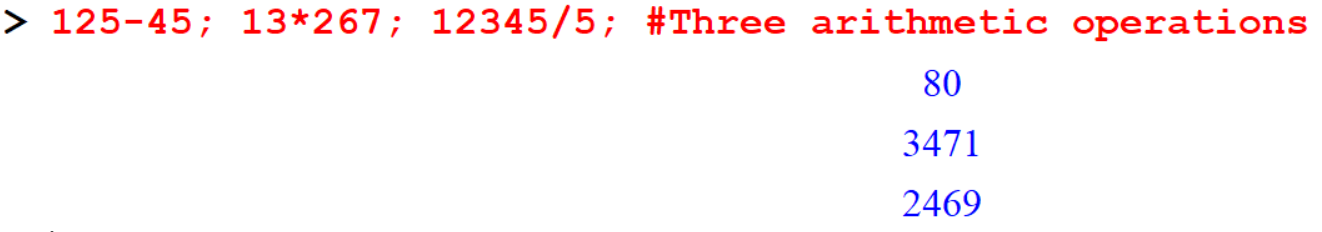
\includegraphics{figures/Lesson 1/fig9.png}

\begin{verbatim}
[> 2^5;
\end{verbatim}

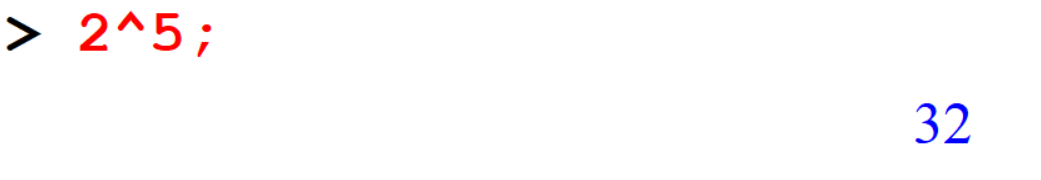
\includegraphics{figures/Lesson 1/fig10.png}

\begin{verbatim}
[> 2^(-5);
\end{verbatim}

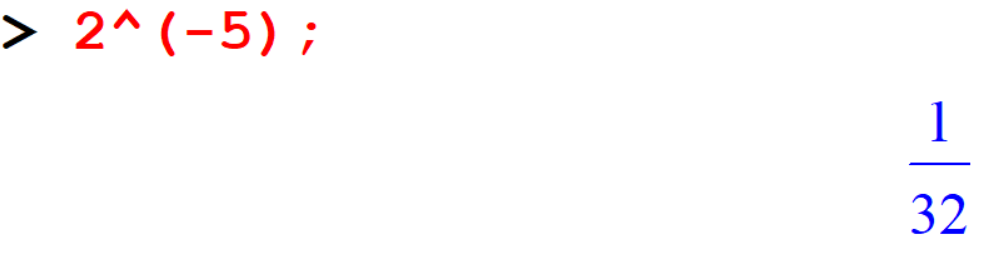
\includegraphics{figures/Lesson 1/fig11.png}

\begin{verbatim}
[> 3^40;
\end{verbatim}

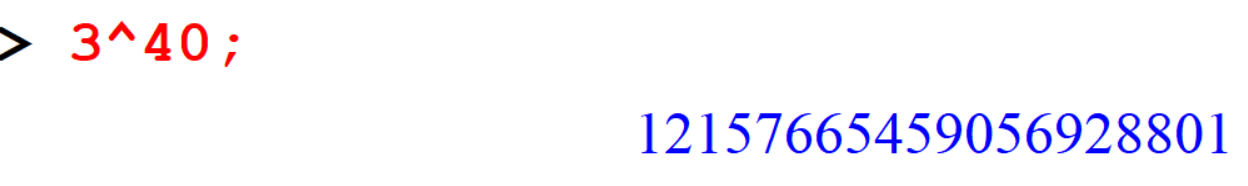
\includegraphics{figures/Lesson 1/fig12.png}

\begin{remark}
\textbf{\emph{Don't use commas when you type large numbers in Maple.
- For example: Compute the product 102,136,543 \& 20,077,410 .}}
\end{remark}

\begin{verbatim}
[> 102136543*20077410;
\end{verbatim}

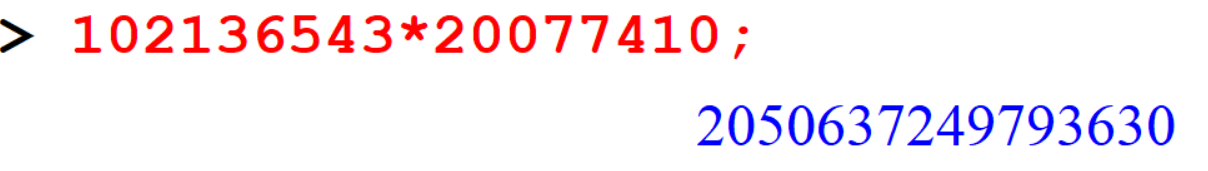
\includegraphics{figures/Lesson 1/fig13.png}

\section{Operations}\label{operations}

Maple adheres to the same order of operations that we use in Mathematics. By inserting parentheses, we can change this order.

\begin{verbatim}
[> 2+3*4-5*6;
[> 2+(3*4-5)*6;
[> (2+3)*4-5*6;
\end{verbatim}

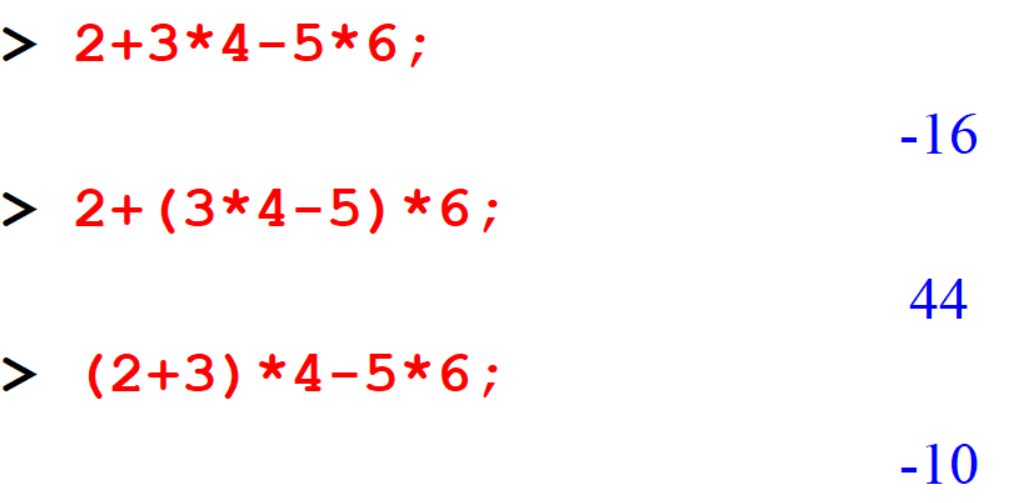
\includegraphics{figures/Lesson 1/fig14.png}

\begin{verbatim}
[> 29/(100-11*3^2);
\end{verbatim}

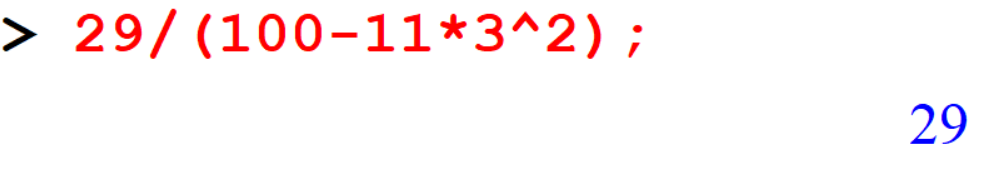
\includegraphics{figures/Lesson 1/fig15.png}

\begin{verbatim}
[> (3^4-2^6)/(3^2-2^3);
\end{verbatim}

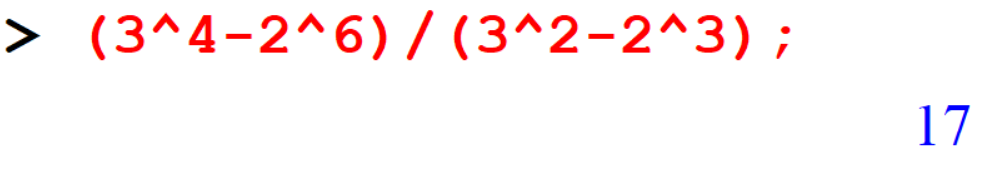
\includegraphics{figures/Lesson 1/fig16.png}

\subsection{Exercises}\label{exercises}

\begin{exercise}
\protect\hypertarget{exr:unnamed-chunk-2}{}\label{exr:unnamed-chunk-2}\leavevmode

\begin{enumerate}
\def\labelenumi{\arabic{enumi}.}
\tightlist
\item
  Calculate the followings
\end{enumerate}

\begin{enumerate}
\def\labelenumi{\roman{enumi}.}
\tightlist
\item
  \(1428 + 456 − 41\)
\item
  \(421 × 240 ÷ 55\)
\item
  \((128 − 691 + 458) × 8\)
\item
  \(2214875(201 × 11 − 55)\)
\item
  \(201 ÷ (2012 − 1)\)
\item
  \(21^{4^{2^3}}\)
\end{enumerate}

\end{exercise}

\begin{exercise}
\protect\hypertarget{exr:unnamed-chunk-3}{}\label{exr:unnamed-chunk-3}\leavevmode

\begin{enumerate}
\def\labelenumi{\roman{enumi}.}
\tightlist
\item
  Compute \(3^{400}\).
\item
  Find the command to find the length (number of digits) of a number.
\item
  How many digits are there in the number \(3^{400}\) ?
\item
  Does the above command give correct answer to the fractional numbers?
\end{enumerate}

\end{exercise}

\section{Shortcut to retyping}\label{shortcut-to-retyping}

One shortcut that we use often in Maple to retype is the \texttt{\%} key. This refers to most recently executed result.

\begin{verbatim}
[> 13*23+1;
[> %/5;
[> %%/5;
[> %%%/5;
\end{verbatim}

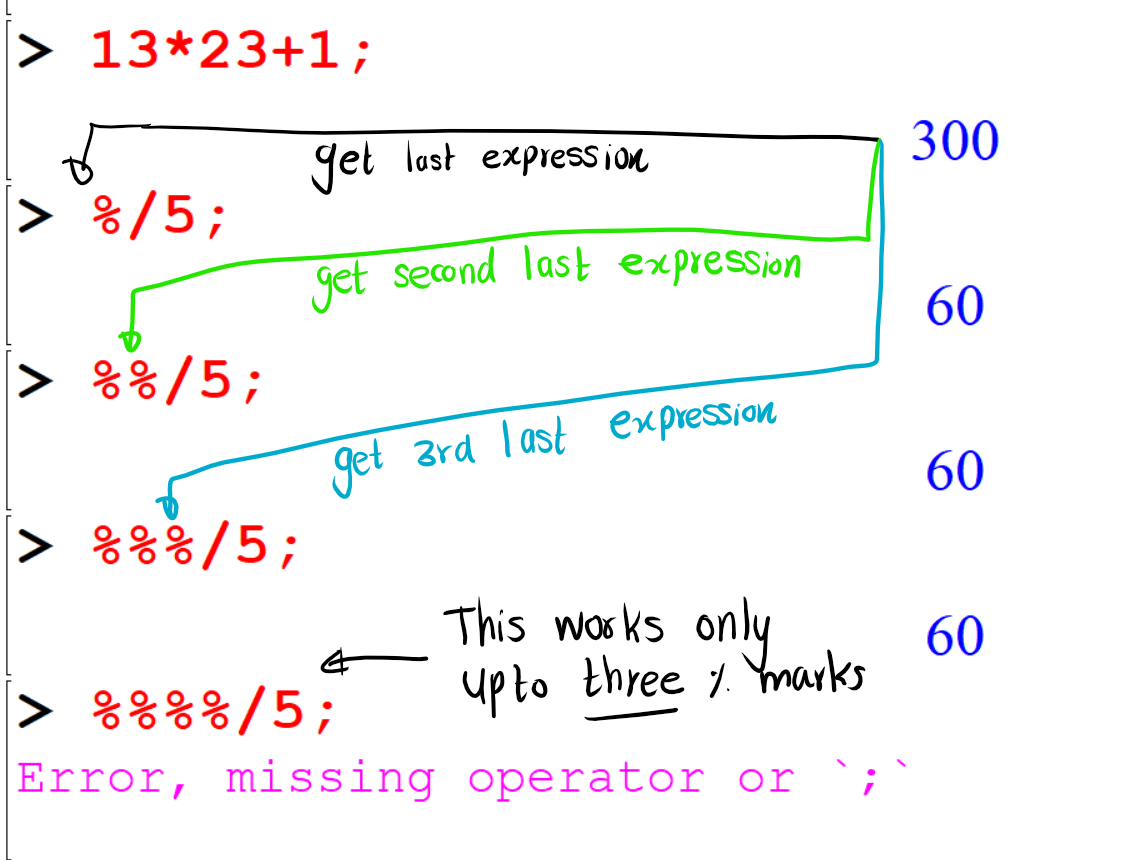
\includegraphics{figures/Lesson 1/fig17.png}

\begin{verbatim}
[> 12540*4;
[> %/4;
[> %/4;
\end{verbatim}

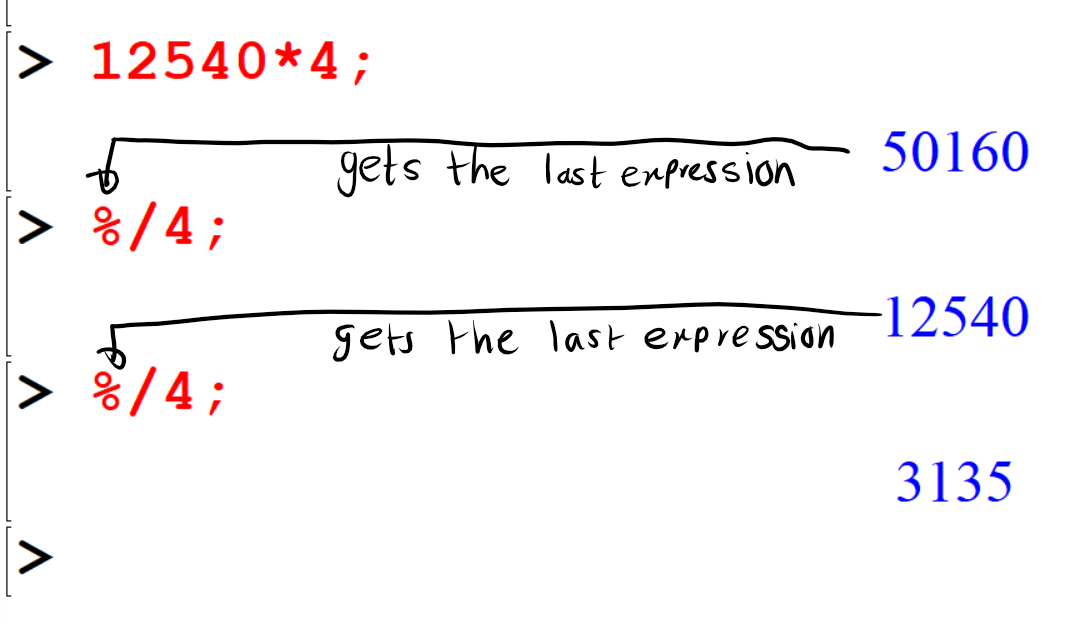
\includegraphics{figures/Lesson 1/fig18.png}

\section{Fractions and Decimals}\label{fractions-and-decimals}

By simply entering a fraction Maple automatically reduce it.

\begin{verbatim}
[> 45/4;
\end{verbatim}

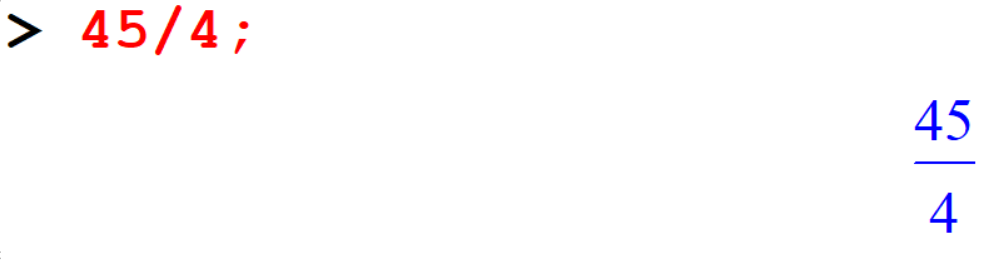
\includegraphics{figures/Lesson 1/fig19.png}

\begin{verbatim}
[> 148/24;
\end{verbatim}

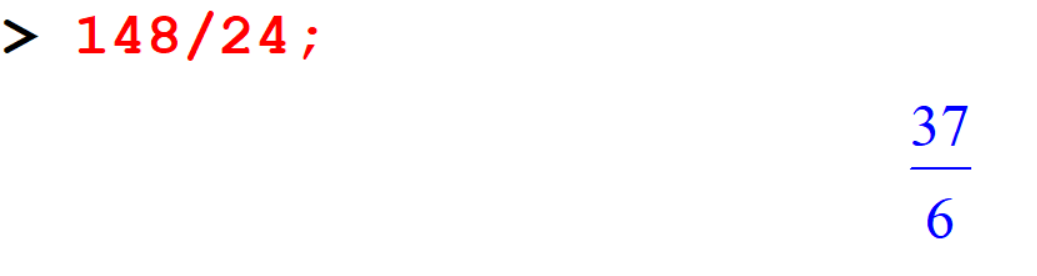
\includegraphics{figures/Lesson 1/fig20.png}

\begin{verbatim}
[> 25/15;
\end{verbatim}

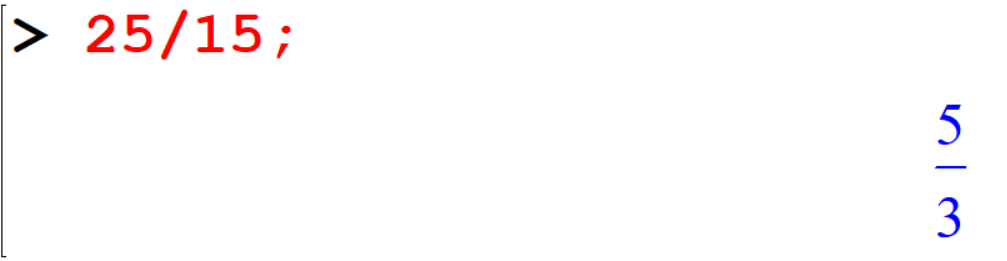
\includegraphics{figures/Lesson 1/fig21.png}

\begin{verbatim}
[> 2/3+3/7;
\end{verbatim}

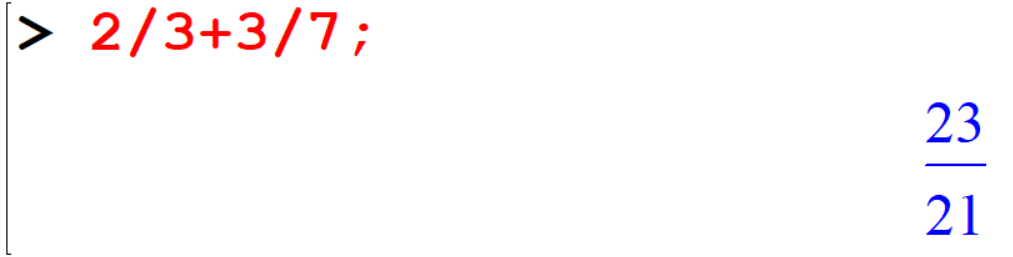
\includegraphics{figures/Lesson 1/fig22.png}

\begin{verbatim}
[> 3/2+4/5-1/3;
\end{verbatim}

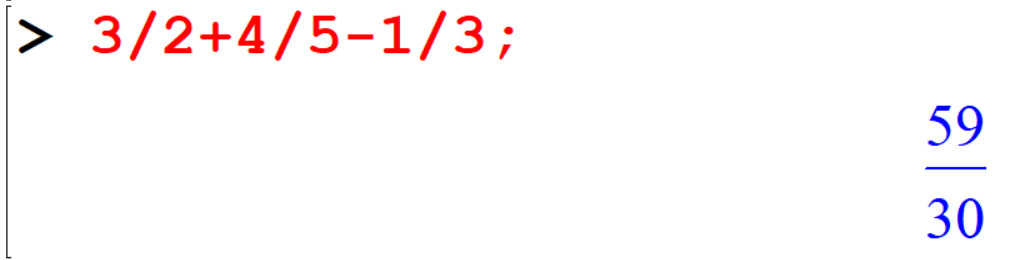
\includegraphics{figures/Lesson 1/fig23.png}
You can do calculations with decimal numbers also.

\begin{verbatim}
[> 25.361+124.6;
\end{verbatim}

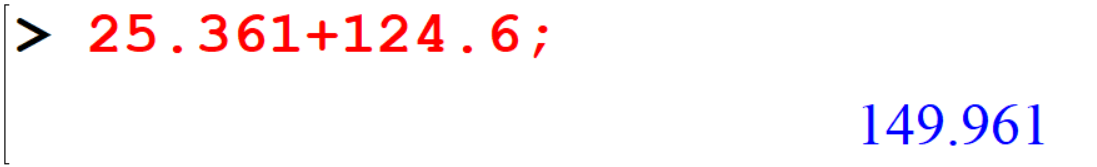
\includegraphics{figures/Lesson 1/fig24.png}

\begin{verbatim}
[> 2.138*0.013;
\end{verbatim}

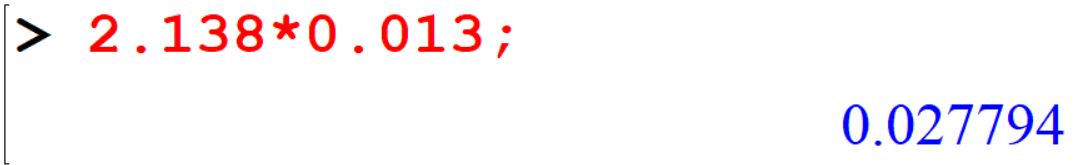
\includegraphics{figures/Lesson 1/fig25.png}

\begin{verbatim}
[> 56.101/0.102;
\end{verbatim}

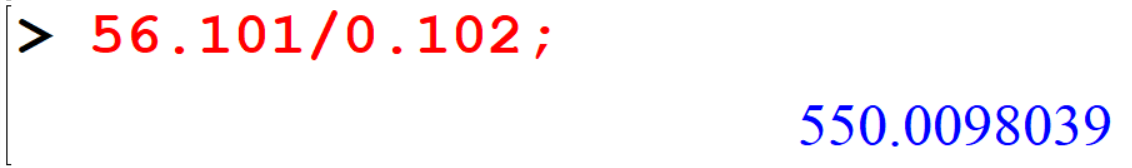
\includegraphics{figures/Lesson 1/fig26.png}

\section{Roots}\label{roots}

\begin{verbatim}
[> sqrt(16);
\end{verbatim}

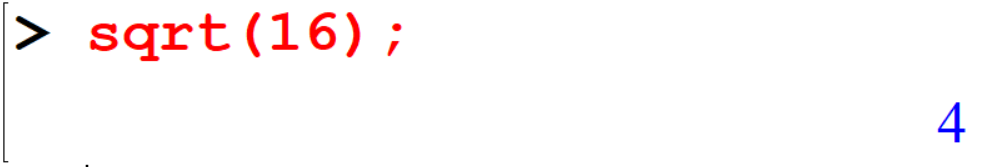
\includegraphics{figures/Lesson 1/fig27.png}

\begin{verbatim}
[> sqrt(30);
\end{verbatim}

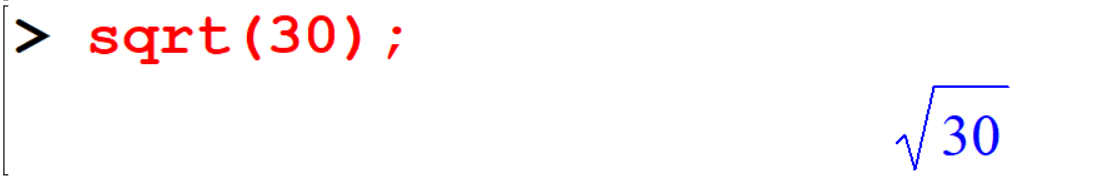
\includegraphics{figures/Lesson 1/fig28.png}

\begin{verbatim}
[> evalf(sqrt(30));
\end{verbatim}

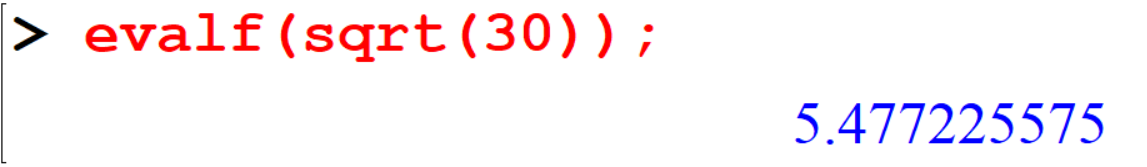
\includegraphics{figures/Lesson 1/fig29.png}

\begin{quote}
The \texttt{evalf} command numerically evaluates expressions (or sub-expressions) involving constants (for example, \texttt{Pi}, \texttt{exp(1)}) and mathematical functions (for example, \texttt{exp}, \texttt{ln}, \texttt{sin}).
\end{quote}

\begin{verbatim}
[> 30^(1/2);
[> evalf(%);
\end{verbatim}

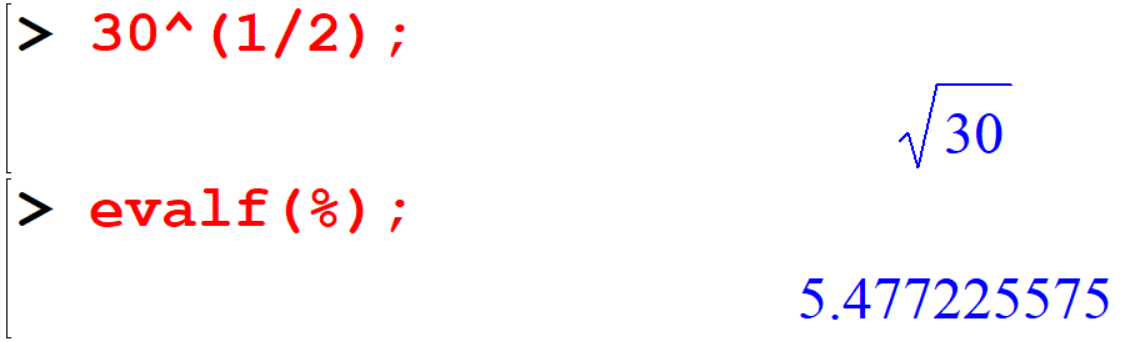
\includegraphics{figures/Lesson 1/fig30.png}

\subsection{Exercise}\label{exercise}

\begin{exercise}
\protect\hypertarget{exr:unnamed-chunk-4}{}\label{exr:unnamed-chunk-4}

Compute the following:

\begin{enumerate}
\def\labelenumi{\roman{enumi}.}
\tightlist
\item
  \(11 + \sqrt{31}\)
\item
  \(\sqrt[3]{64}\)
\item
  \(\sqrt{2}^{\sqrt{3}}\)
\end{enumerate}

\end{exercise}

\begin{exercise}
\protect\hypertarget{exr:unnamed-chunk-5}{}\label{exr:unnamed-chunk-5}

Calculate \(120^8\)

\begin{enumerate}
\def\labelenumi{\roman{enumi}.}
\tightlist
\item
  Divide the answer by \(10^8\)
\item
  Divide the answer in part i. by \(2048 \times 8\)
\end{enumerate}

\end{exercise}

\section{Pi Vs pi}\label{pi-vs-pi}

\(\pi\) is a constant in Mathematics and is recognized by maple and typed as \texttt{Pi} \textbf{(Note the capitalization of ``p'' but not ``i')}.

\begin{verbatim}
[> Pi;
[> evalf(%);
\end{verbatim}

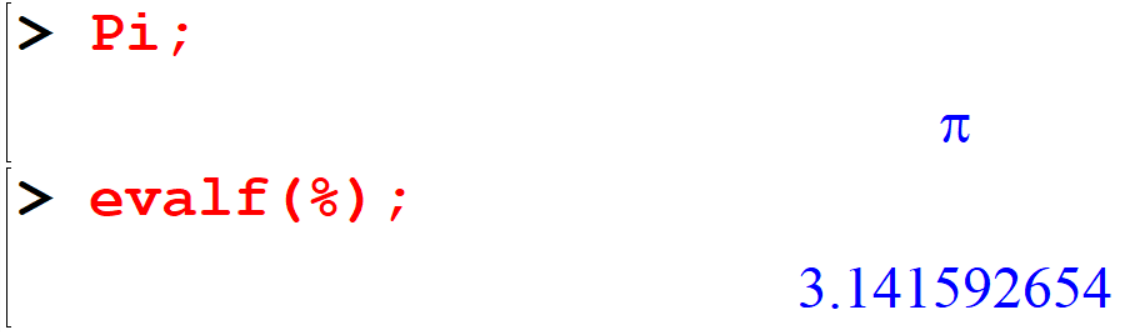
\includegraphics{figures/Lesson 1/fig31.png}

\begin{verbatim}
[> evalf(2*Pi);
\end{verbatim}

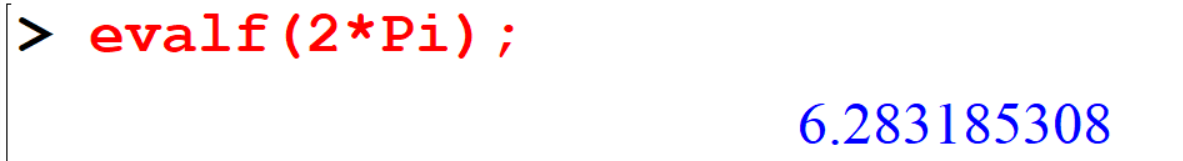
\includegraphics{figures/Lesson 1/fig32.png}
If you use \texttt{pi} then \texttt{evalf} command does not return \(\pi\) numerically.

\begin{verbatim}
[> pi;
[> evalf(%);
\end{verbatim}

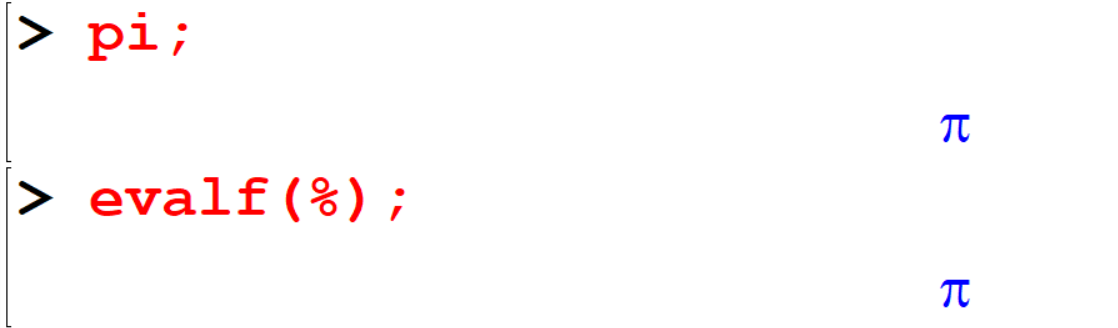
\includegraphics{figures/Lesson 1/fig33.png}

\section{Rational Numbers}\label{rational-numbers}

Maple usually leaves fractions in fraction form. However, we can force it to express fractions in decimal form using the \texttt{evalf} command.

\begin{verbatim}
[> 1/7;
[> evalf(1/7);
\end{verbatim}

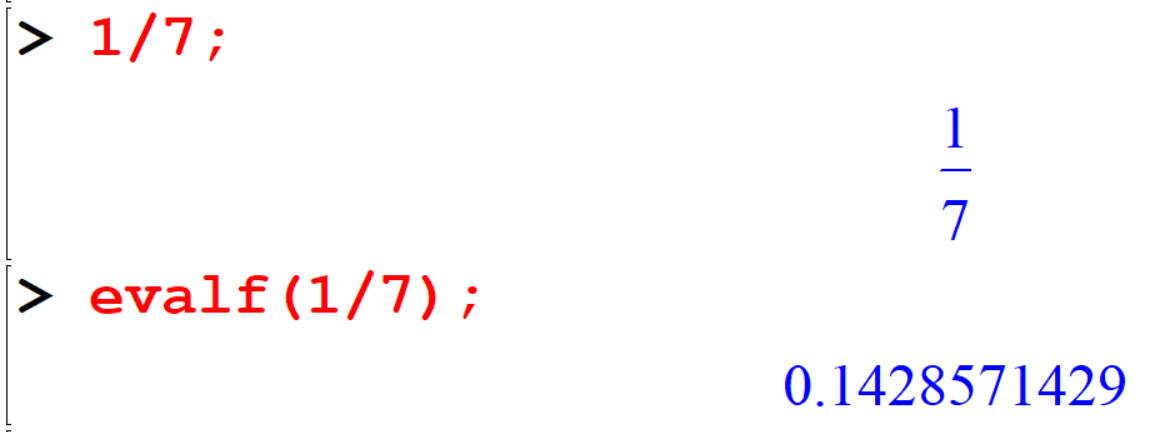
\includegraphics{figures/Lesson 1/fig34.png}

\begin{verbatim}
[> 25/35;
[> evalf(%);
\end{verbatim}

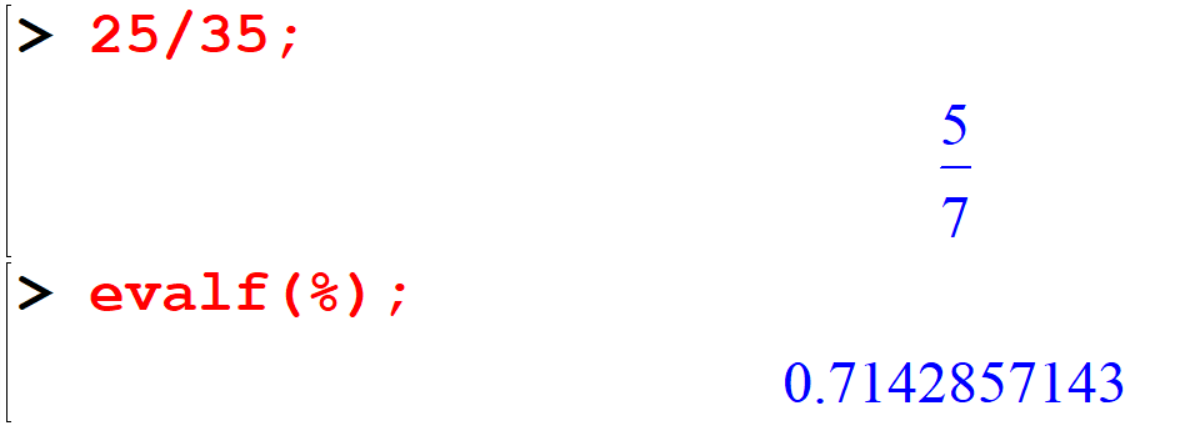
\includegraphics{figures/Lesson 1/fig35.png}

Maple displays 10 decimal places as a default. If this is not enough and for better precision you can specify the exact number of decimal places as a second parameter to the \texttt{evalf} command.

Note that the second parameter normally represents the number of non-zero digits in the answer.

\begin{verbatim}
[> evalf(1/7,100);
\end{verbatim}

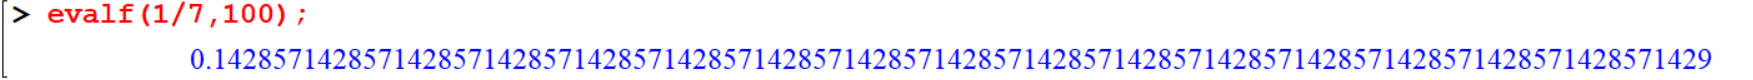
\includegraphics{figures/Lesson 1/fig36.png}

\begin{verbatim}
[> evalf(29/3,5);
\end{verbatim}

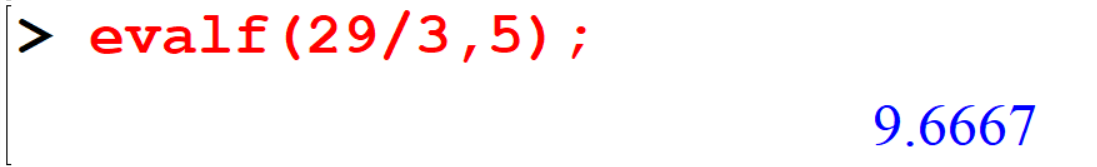
\includegraphics{figures/Lesson 1/fig37.png}

Here, if you want to calculate the answer for 4 decimal places the command should be \texttt{evalf(29/3,5)} and if you want the answer to be 5 decimal places the command should be \texttt{evalf(29/3,6)}.

\begin{verbatim}
[> evalf(1/15,5);
\end{verbatim}

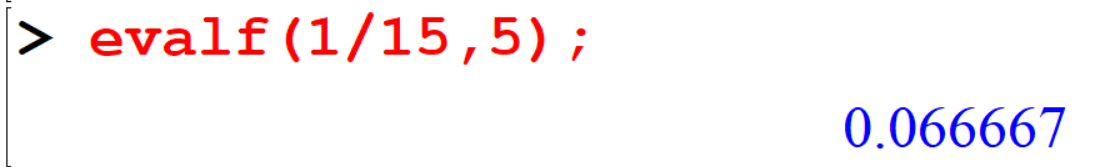
\includegraphics{figures/Lesson 1/fig38.png}

\begin{verbatim}
[> evalf(11/19,5);
\end{verbatim}

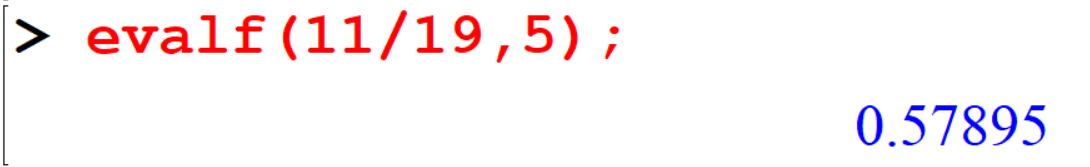
\includegraphics{figures/Lesson 1/fig39.png}
Fractions are also rational numbers because their decimal expansions always have repeating blocks of digits. By looking at the decimal representation of a rational number you can see the repeating cycle.

\begin{verbatim}
[> evalf(1/35);
\end{verbatim}

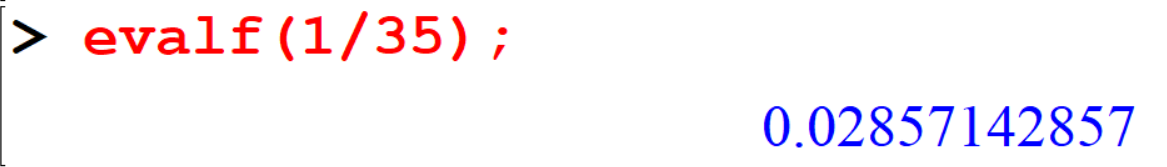
\includegraphics{figures/Lesson 1/fig40.png}
Here we can not see the repeat cycle. But if we calculate \(\frac{1}{35}\) for more decimal places we can see the repeating cycle.

\begin{verbatim}
[> evalf(1/35, 100);
\end{verbatim}

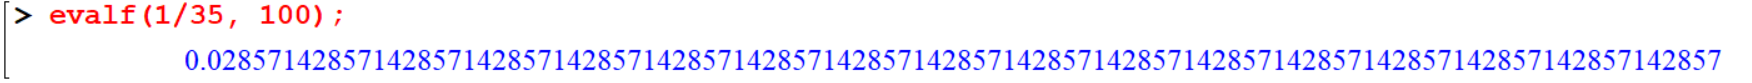
\includegraphics{figures/Lesson 1/fig41.png}

\subsection{Exercises}\label{exercises-1}

\begin{exercise}
\protect\hypertarget{exr:unnamed-chunk-6}{}\label{exr:unnamed-chunk-6}Evaluate the value of π correct up to 5 decimal places.
\end{exercise}

\begin{exercise}
\protect\hypertarget{exr:unnamed-chunk-7}{}\label{exr:unnamed-chunk-7}Find the area of a circle with radius 10cms
\end{exercise}

\begin{exercise}
\protect\hypertarget{exr:unnamed-chunk-8}{}\label{exr:unnamed-chunk-8}

Check whether the followings are rational numbers or not

\begin{enumerate}
\def\labelenumi{\roman{enumi}.}
\tightlist
\item
  \(\frac{1}{49}\)
\item
  \(\pi\)
\item
  \(\sqrt{2}\)
\end{enumerate}

\end{exercise}

\begin{exercise}
\protect\hypertarget{exr:unnamed-chunk-9}{}\label{exr:unnamed-chunk-9}How many digits are repeating in \(\frac{1}{212}\)
\end{exercise}

\section{Complex Numbers}\label{complex-numbers}

In Maple, complex arithmetic is normally done automatically with \texttt{I} standing for \(\sqrt{−1}\) (for example, if you square \texttt{I} you will get \texttt{-1}, not \texttt{I\^{}2})

\begin{verbatim}
[> (-4+7*I)+(5-10*I);
\end{verbatim}

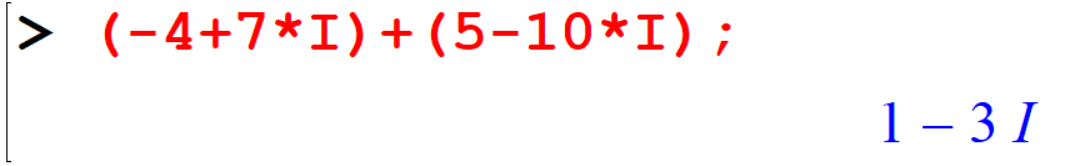
\includegraphics{figures/Lesson 1/fig42.png}

\begin{verbatim}
[> 5*I-(-9+I);
\end{verbatim}

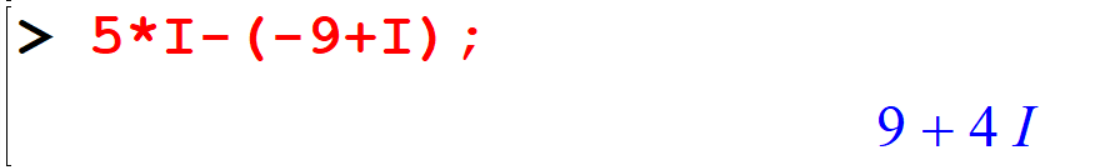
\includegraphics{figures/Lesson 1/fig43.png}

\begin{verbatim}
[> (1-5*I)*(-9+2*I);
\end{verbatim}

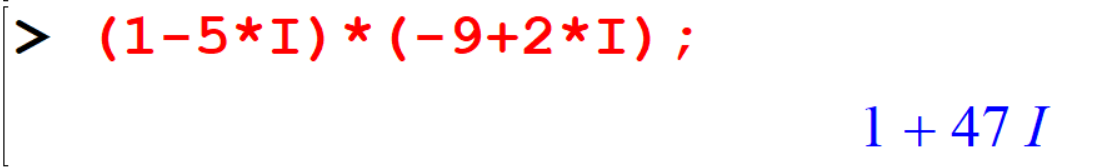
\includegraphics{figures/Lesson 1/fig44.png}

\begin{verbatim}
[> (3-I)/(2+7*I);
\end{verbatim}

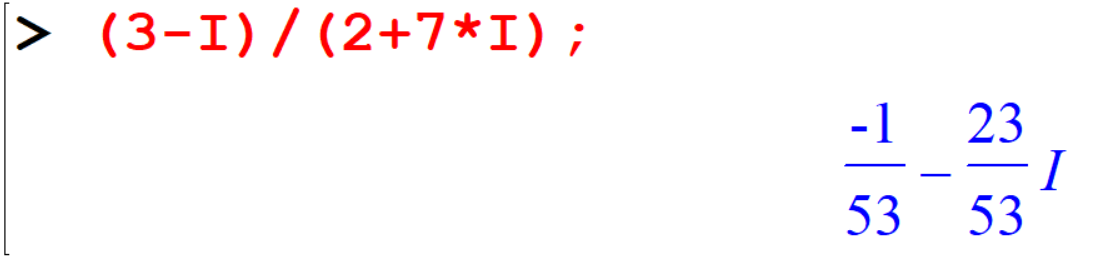
\includegraphics{figures/Lesson 1/fig45.png}
But Maple does not always automatically evaluate an expression involving complex numbers.
For example, it may leave an expression as the product of some complex numbers or as an expression involving a root of a complex number.

\begin{verbatim}
[> (-2*I)^(1/2);
\end{verbatim}

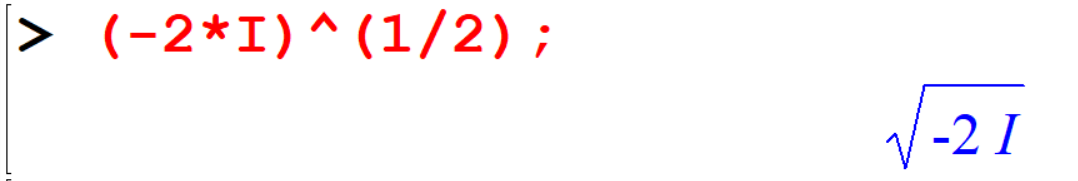
\includegraphics{figures/Lesson 1/fig46.png}
The function \texttt{evalc} to force Maple to evaluate as a complex number.

\begin{verbatim}
[> evalc((-2*I)^(1/2));
\end{verbatim}

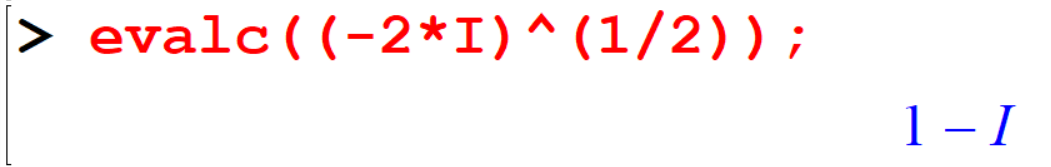
\includegraphics{figures/Lesson 1/fig47.png}
Note that \texttt{evalc} does not give you both the square roots of \texttt{-2*I} it only gives the \emph{principal value} of the root.

If you want to find the roots, use solve command as follows.

\begin{verbatim}
[> solve(z^2=-2*I);
\end{verbatim}

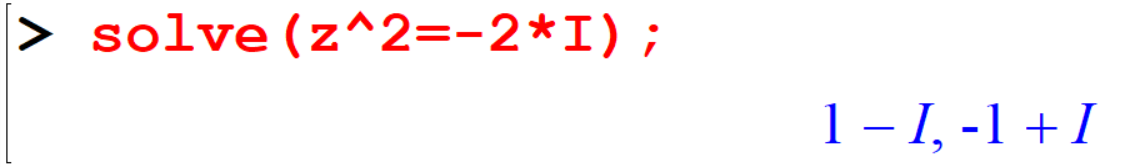
\includegraphics{figures/Lesson 1/fig48.png}

\subsection{Exercise}\label{exercise-1}

\begin{exercise}
\protect\hypertarget{exr:unnamed-chunk-10}{}\label{exr:unnamed-chunk-10}

Simplify the following:

\begin{enumerate}
\def\labelenumi{\arabic{enumi}.}
\tightlist
\item
  \((−3 + 3i) + (7 – 2i)\)
\item
  \((5 + 3i) − (3 − i)\)
\item
  \((1 + 2i)(1 − 2i) 4. (56 − 8i) ÷ (14 + 10i)\)
\end{enumerate}

\end{exercise}

\begin{exercise}
\protect\hypertarget{exr:unnamed-chunk-11}{}\label{exr:unnamed-chunk-11}\leavevmode

\begin{enumerate}
\def\labelenumi{\arabic{enumi}.}
\setcounter{enumi}{1}
\tightlist
\item
  Simplify \((2i)^\frac{1}{2}\) by using \texttt{evalc} and solve commands.
\end{enumerate}

\end{exercise}

\begin{exercise}
\protect\hypertarget{exr:unnamed-chunk-12}{}\label{exr:unnamed-chunk-12}\leavevmode

\begin{enumerate}
\def\labelenumi{\arabic{enumi}.}
\setcounter{enumi}{2}
\tightlist
\item
  Multiply the following and obtain the answer in standard form:
  \[(2 − \sqrt{−100})(1 + \sqrt{−36})\]
\end{enumerate}

\end{exercise}

\section{MAPLE Help}\label{maple-help}

Maple contains a complete online help system you can use to find information about specific topic easily and to explore the wide range of commands available. To get the information about commands, which you learn in MAPLE, you can use either one of the following.

\begin{itemize}
\tightlist
\item
  Topic search function
\item
  F1 key
\item
  \texttt{?} In front of the command
\end{itemize}

\chapter{Basic Algebra}\label{basic-algebra}

\section{Variables and Expressions}\label{variables-and-expressions}

Study how we write the following expressions in Maple.

\begin{verbatim}
[> 3*x;
\end{verbatim}

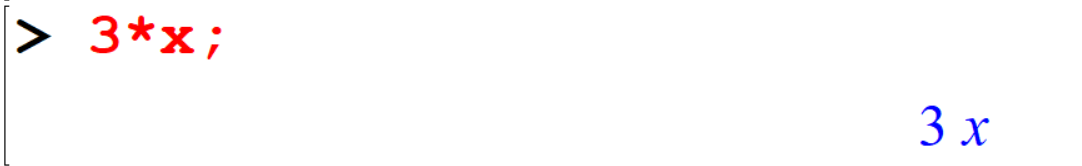
\includegraphics{figures/Lesson 1/fig50.png}

\begin{verbatim}
[> 2+3*x;
\end{verbatim}

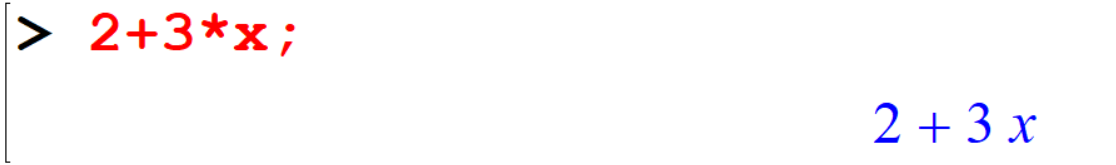
\includegraphics{figures/Lesson 1/fig51.png}

\begin{verbatim}
[> x^2;
\end{verbatim}

\includegraphics{figures/Lesson 1/fig52.png}

\begin{verbatim}
[> 1/(x-2);
\end{verbatim}

\includegraphics{figures/Lesson 1/fig53.png}

\subsection{Exercise}\label{exercise-2}

\begin{exercise}
\protect\hypertarget{exr:unnamed-chunk-13}{}\label{exr:unnamed-chunk-13}

Generate the following expressions using maple commands.

\begin{enumerate}
\def\labelenumi{\roman{enumi})}
\tightlist
\item
  \((2x + 3)(4x + 5)\)
\item
  \(9x^2 − 4\)
\item
  \(\frac{2x}{5}+\frac{y}{5}\)
\item
  \(\frac{\sqrt{2x+1}}{3+y}\)
\end{enumerate}

\end{exercise}

\section{Assigning values to variables}\label{assigning-values-to-variables}

Maple will store things (numbers, expressions, functions,\ldots) in `containers' or `variables'.
This process is called assignment, and you can assign values to the variables by using \texttt{:=} or using the command \texttt{assign}. After assigning a value to a variable it becomes a constant and Maple will remember that value from that point.

\begin{itemize}
\tightlist
\item
  \textbf{Method I}
\end{itemize}

\begin{verbatim}
[> x:=5;
\end{verbatim}

\begin{verbatim}
[> x^2;
\end{verbatim}

\begin{verbatim}
[> 2*x+23;
\end{verbatim}

\includegraphics{figures/Lesson 1/fig56.png}

\begin{itemize}
\tightlist
\item
  \textbf{Method II}
\end{itemize}

\begin{verbatim}
[> assign(y,5);
\end{verbatim}

\begin{verbatim}
[> y^2;
\end{verbatim}

\includegraphics{figures/Lesson 1/fig57.png}

\begin{quote}
You can also define variables in a descriptive manner. However they must begin with a character and any blank spaces must not be included. Note that maple is case sensitive.
\end{quote}

\begin{verbatim}
[> Age:=21;
\end{verbatim}

\begin{verbatim}
[> age;
\end{verbatim}

\begin{verbatim}
[> Age;
\end{verbatim}

\begin{verbatim}
[> Exam_No:=2012300;
\end{verbatim}

\begin{verbatim}
[> New Age:=Age+4; # There should not be any blank spaces when giving a name for the variable
\end{verbatim}

\begin{verbatim}
[> New_Age:=Age+4;
\end{verbatim}

If you want to reset the predefined value for variables you have to use following methods.

\begin{itemize}
\tightlist
\item
  \textbf{Method I}: \texttt{restart} command\\
\end{itemize}

\begin{verbatim}
[> restart;
[> Age;
\end{verbatim}

\begin{itemize}
\tightlist
\item
  \textbf{Method II} : \texttt{unassign}\\
  The \texttt{unassign} command unassigns all the unevaluated names given as input.
\end{itemize}

\begin{verbatim}
[> x:=5;
[> x+20;
[> unassign('x');
[> x+20;
\end{verbatim}

\section{Substituting Values}\label{substituting-values}

To substitute numbers (or other expressions) in the place of variables in an algebraic expression without permanently changing the values of the variable, we use the command,
\texttt{subs(variable,\ expression)}.

Try to use help

\begin{verbatim}
[> ?subs
\end{verbatim}

\begin{verbatim}
> x;
> subs(x=2,x+5);
> subs(x=2,x^2-5*x+4);
\end{verbatim}

It is convenient to make substitution by giving name for an expression.

\begin{verbatim}
> expr:=(2*x+1)/(5-3*x);
> subs(x=3,expr);
\end{verbatim}

You can even substitute other variables or expressions to a variable in an expression.

\begin{verbatim}
> subs(x=a,expr);
> subs(x=a+1,expr);
\end{verbatim}

You can also substitute more than one variable for a expression.

\begin{verbatim}
[> expr1:=(7*x-3*y)/(x^2-y^2);
\end{verbatim}

\begin{verbatim}
[> subs({x=3,y=2},expr1);
\end{verbatim}

\begin{verbatim}
[> subs({x=a-2,y=a+2},expr1);
\end{verbatim}

\begin{verbatim}
[> expr2:=x^2+2*y^2+z^2;
\end{verbatim}

\begin{verbatim}
[> subs({x=1,y=2,z=3},expr2);
\end{verbatim}

\section{Factoring expressions}\label{factoring-expressions}

Maple can factorize an integer into primes using the command \texttt{ifactor}.

\begin{verbatim}
[> ifactor(18);
\end{verbatim}

\begin{verbatim}
[> ifactor(525);
\end{verbatim}

\begin{verbatim}
[> ifactor(2^8-1);
\end{verbatim}

\section{Expanding expressions}\label{expanding-expressions}

One of the most important things Maple can do is to calculate with expressions as well as numbers and we use the command \texttt{expand} to get the expansion of an expression.

\section{Finding the degree and leading coefficient of polynomials}\label{finding-the-degree-and-leading-coefficient-of-polynomials}

The highest power of the variable that occurs in the polynomial is called the \textbf{degree} of a polynomial.
The \textbf{leading term} is the term with the highest power, and its coefficient is called the \textbf{leading coefficient}.

If \(x\) is a single indeterminate, the \texttt{degree} and \texttt{ldegree} commands compute the degree and low degree respectively, of the polynomial \(p\) in \(x\).

\begin{verbatim}
[> p:=(x+5)^5;
[> expand(%);
[> degree(p,x);
[> ldegree(p,x);
\end{verbatim}

\includegraphics{figures/Lesson 1/fig54.png}

The \texttt{coeff(p,\ x\^{}n)} command finds the coefficient of \(x^n\) in the polynomial \(p\) where \(p\) is the
polynomial in \(x\) and \(n\) is the integer corresponds to the power. When finding the leading coefficient, \(n\) corresponds to the highest power in the polynomial.

\begin{verbatim}
[> coeff(p,x^5);
\end{verbatim}

\begin{verbatim}
[> coeff(p,x,5); #Another way of finding leading coefficient
\end{verbatim}

\includegraphics{figures/Lesson 1/fig55.png}

\subsection{Exercise}\label{exercise-3}

\begin{exercise}
\protect\hypertarget{exr:unnamed-chunk-14}{}\label{exr:unnamed-chunk-14}Generate the expression \(x^3 + \sqrt{x}\) using maple commands and find the value of the expression when \(x = 4\).
\end{exercise}

\begin{exercise}
\protect\hypertarget{exr:unnamed-chunk-15}{}\label{exr:unnamed-chunk-15}\(PQR\) is an isosceles triangle where \(𝑄 = 𝑃𝑅 = 2𝑟 + 3\) and \(𝑄𝑅 = 𝑟 + 3\). Find an expression for the perimeter of the \(𝑃𝑄𝑅\) triangle in terms of \(𝑟\), giving your answer in its simplest form and find the perimeter when \(𝑟 = 8\).
\end{exercise}

\begin{exercise}
\protect\hypertarget{exr:unnamed-chunk-16}{}\label{exr:unnamed-chunk-16}

Factorize the following expressions:

\begin{enumerate}
\def\labelenumi{\roman{enumi}.}
\tightlist
\item
  \(3x^2 + 8x + 5\)
\item
  \(x^4 − 3x^2 + 2\)
\item
  \(36^{13}𝑏^{10} − 40𝑎^{11}𝑏^{11}\)
\item
  \(24389x^{12} − 2197\)
\end{enumerate}

\end{exercise}

\begin{exercise}
\protect\hypertarget{exr:unnamed-chunk-17}{}\label{exr:unnamed-chunk-17}

Expand the following expressions, find the degree, lower degree and the leading coefficients.

\begin{enumerate}
\def\labelenumi{\roman{enumi}.}
\tightlist
\item
  \((5x − 11)^{13}\)
\item
  \((x^2 + x + 1)\)\^{}\{10\})
\end{enumerate}

\end{exercise}

\section{Simplifying Expressions}\label{simplifying-expressions}

2.7 Simplifying Expressions

\begin{verbatim}
[> 3*(x-1)+7*(x+2)-5*(x+11);
\end{verbatim}

Maple will automatically simplify some simple expressions. However, more complicated expressions will not be simplified. So, we need to give a command to simplify such expressions.

\begin{verbatim}
[> 3*(x-1)^2+7*(x+2)^3-5*(x+11)^4;
[> %=simplify(%);
\end{verbatim}

\begin{verbatim}
[> simplify((x^2-y^2)/(x-y));
\end{verbatim}

\chapter{Equations and Functions}\label{equations-and-functions}

\section{Solving Equations}\label{solving-equations}

In general we can solve different types of equations to get an exact solution. The solution may be an integer, a fraction, or it may be an expression. Using Maple we can do the same thing using the \texttt{solve} command and obtain an exact solutions for equations and inequalities.

\section{Equations with multiple unknowns}\label{equations-with-multiple-unknowns}

You can use the solve command to solve equations having several variables. However you have to specify, for which variable that the equation to be solved.

\section{Functions}\label{functions}

Let \(f\) be a function of \(x\). We denote it as \(f(x)\), but in Maple there is a different way to define such functions.

\subsection{Defining functions}\label{defining-functions}

\subsection{Function Operations and Compositions}\label{function-operations-and-compositions}

\subsection{Composition of functions}\label{composition-of-functions}

\section{Trigonometry with Maple}\label{trigonometry-with-maple}

\begin{itemize}
\tightlist
\item
  The Trigonometric functions
\end{itemize}

\[
\begin{aligned}
 \sin(x) && \cos(x) && \tan(x) \\
 \sec(x) && \csc(x) && \cot(x)
\end{aligned}
\]

\begin{itemize}
\tightlist
\item
  The Hyperbolic functions
\end{itemize}

\[
\begin{aligned}
 \sinh(x) && \cosh(x) && \tanh(x) \\
 \text{sech}(x) &&  \text{csch}(x) && \text{coth}(x) 
\end{aligned}
\]

\section{Inverse trigonometric functions}\label{inverse-trigonometric-functions}

\[
\begin{aligned}
 &\arcsin(x)        && \arccos(x)  && \arctan(x)\\
 &\text{arcsec}(x)  && \text{arccsc}(x)  && \text{arccot}(x)\\
 &\text{arcsinh}(x) && \text{arccosh}(x) && \text{arctanh}(x)\\
 &\text{arcsech}(x) && \text{arccsch}(x) && \text{arccoth}(x)
\end{aligned}
\]

\section{Exercise}\label{exercise-4}

\begin{exercise}
\protect\hypertarget{exr:unnamed-chunk-18}{}\label{exr:unnamed-chunk-18}

Find the solutions of the following equations to 5 decimal places.

\begin{enumerate}
\def\labelenumi{\roman{enumi}.}
\tightlist
\item
  \(2x^3 + 3x + 1 = 0\)
\item
  \(2x^3 + 3x + \frac{1}{4} = 0\)
\item
  \(x^2 - 13x + 10 = 0\)
\item
  \(-3x + \frac{1}{2}x^2 = 25\)
\end{enumerate}

\end{exercise}

\begin{exercise}
\protect\hypertarget{exr:unnamed-chunk-19}{}\label{exr:unnamed-chunk-19}

Find the most accurate real solutions to the following equations.

\begin{enumerate}
\def\labelenumi{\roman{enumi}.}
\tightlist
\item
  \(x^4 - 2x^3 = 7\)
\item
  \(\frac{7}{(x-3)^2} + \frac{5}{(x+5)}\)
\end{enumerate}

\end{exercise}

\begin{exercise}
\protect\hypertarget{exr:unnamed-chunk-20}{}\label{exr:unnamed-chunk-20}Express the following in the form of \(y =mx +c\) using the \texttt{solve} command.

\begin{enumerate}
\def\labelenumi{\roman{enumi}.}
\tightlist
\item
  \(3x + 4y = 2\)
\item
  \(\frac{3y}{5} - 2x + 7 = 0\)
\item
  \(\frac{x}{x-3} + \frac{y}{2x} = -3\)
\end{enumerate}

Use the Maple help to find another way to do the above.\\
(Hint: You have to \texttt{isolate} y in each equation.)
\end{exercise}

\begin{exercise}
\protect\hypertarget{exr:unnamed-chunk-21}{}\label{exr:unnamed-chunk-21}

Consider, \(f(x) = 2x -\frac{x}{3(x+1)}\)

\begin{enumerate}
\def\labelenumi{\roman{enumi}.}
\tightlist
\item
  Define \(f\) as a function: \(f(x) = 2x - \frac{x^3}{x+1}\)
\item
  Evaluate \(f(-\frac{1}{2})\)
\item
  Factor \(f(x)\)
\item
  Simplify \(f(\frac{1}{t-1})\)
\end{enumerate}

\end{exercise}

\begin{exercise}
\protect\hypertarget{exr:unnamed-chunk-22}{}\label{exr:unnamed-chunk-22}

Use Maple help to find out how to find \texttt{logarithms}. Then find the value of the following.

\begin{enumerate}
\def\labelenumi{\roman{enumi}.}
\tightlist
\item
  \(\log_{10} 100\)
\item
  \(\ln 100\)
\item
  \(\log_3 10\)
\item
  \(2\log_3 81 + 5\log_8 256\)
\end{enumerate}

\end{exercise}

\begin{exercise}
\protect\hypertarget{exr:unnamed-chunk-23}{}\label{exr:unnamed-chunk-23}

Find the value of the following trigonometric expressions for given \(x\).

\begin{enumerate}
\def\labelenumi{\roman{enumi}.}
\tightlist
\item
  \(\sin(\sec(x^2)) + 3x\cos^3(\frac{2x}{7})\), where \(x = 71^\circ\).
\item
  \(\sec^{-1}(\tanh(x+5))\cos(\sec(2x) + \sin(2x))\), where \(x = 43^\circ\).
\item
  \(\left(\cot^{-1}(x) + \sec^{-1}(\frac{x-3}{5})\right)^{\frac{1}{3}}\), where \(x = 71^circ\).
\end{enumerate}

\end{exercise}

\chapter{Plots}\label{plots}

\textbf{Maple Packages}

In Maple we can use various packages for special applications. In order to use a package, you have to load the package first using the \texttt{with} command.

\textbf{Example}\\
\texttt{\textgreater{}\ with(student):}\strut \\
\texttt{\textgreater{}\ with(linalg):}

So, when you are dealing with plots, you have to load the package \texttt{plot}.

\begin{verbatim}
 > with(plots):
\end{verbatim}

\section{Basic Graphs}\label{basic-graphs}

Using the plot command you can graph a function. You have to give the range of values for \(x\) otherwise Maple will use the default range.

\section{Multiple Graphs}\label{multiple-graphs}

If you want to compare plots, you can have two or more plot windows open at the same time or you can plot more than one curve on the same set of axes. The plot command offers options which control the number of points at which the function is plotted, the number of
tick marks on the axes and the placing of titles on the graph. Read the help page on plot to find out about these options.

\chapter{Vectors}\label{vectors}

\section{Defining a vector}\label{defining-a-vector}

\chapter{Set Theroy}\label{set-theroy}

\section{Set Definition and Cardinity}\label{set-definition-and-cardinity}

\chapter{Differential Equations}\label{differential-equations}

\section{Introduction to differential equations}\label{introduction-to-differential-equations}

In this Maple session, we see some of the basic tools for working with differential equations in Maple.
First, we need to load the \texttt{DEtools} library:
We can find the derivative of a given function by using \texttt{diff} command.
- The \texttt{diff} command computes the partial derivative of a given expression with respect to the variables given.
- The \texttt{Diff} command returns the unevaluated function. Now consider the following examples.

\begin{example}
\protect\hypertarget{exm:unnamed-chunk-24}{}\label{exm:unnamed-chunk-24}Find the derivative of \(y=xe^x\) with respect to \(x\).
\end{example}

\begin{verbatim}
[> with(DEtools):
[> y:=x->x*exp(-x);
[> Diff(y(x),x);
[> diff(y(x),x);
[> Diff(y(x),x)=diff(y(x),x);
\end{verbatim}

\includegraphics{figures/Diff/Diff 6.1 -1.png}

\begin{example}
\protect\hypertarget{exm:unnamed-chunk-25}{}\label{exm:unnamed-chunk-25}Consider the follwing function \(h\) of two varibels.
\[h(x,y)=5x^2 + 2x^2y + 3xy^2 + 12yx + \frac{3y^3}{x}\]
Now we are going to differentiate \(h\) partially. The next few
commands have been done in order to understand the process.
\end{example}

First, we define the function \(h\).

\begin{verbatim}
[> h :=(x,y)-> 5*x^2+2*x^2*y+3*x*y^2+12*y*x+3*y^3/x;
\end{verbatim}

Then,
\includegraphics{figures/Diff/Diff 6.1 -2.png}

\begin{verbatim}
[> Diff( h(x,y),x);
[> diff( h(x,y),x);
[> Diff( h(x,y),x)=diff( h(x,y),x);
\end{verbatim}

\includegraphics{figures/Diff/Diff 6.1 -3.png}

\begin{verbatim}
[> Diff(h(x,y),y);
[> diff(h(x,y),y);
[> Diff(h(x,y),y)=diff(h(x,y),y);
\end{verbatim}

\includegraphics{figures/Diff/Diff 6.1 -4.png}
Here we are going to differentiate the function \(h\) with respect to \(x\) and \(y\), using them both in one command. Here the function \(h\) should be differentiate first with respect to \(x\), and then again with respect to \(y\).

\begin{verbatim}
[> diff( h(x,y),x,y);
\end{verbatim}

\includegraphics{figures/Diff/Diff 6.1 -5.png}
Now, the function h should be differentiate first with respect to \(y\), and then again with respect to \(x\).

\begin{verbatim}
[> diff( h(x,y),y,x);
\end{verbatim}

\includegraphics{figures/Diff/Diff 6.1 -6.png}
First define the function in Maple. Then you can find the derivative as follows.

\begin{example}
\protect\hypertarget{exm:unnamed-chunk-26}{}\label{exm:unnamed-chunk-26}Define the differential equation \(y' =y(4-y\)
\end{example}

\begin{verbatim}
[> diff(y(t),t) = y(t)*(4-y(t));
\end{verbatim}

\textbf{We cannot drop the `\((t)\)' from the dependent variable \(y\). Maple treats `\(y\)' and `\(y(t)\)' differently, and our equation is for \texttt{\textbackslash{}(y(t)\textbackslash{})}}

\subsection{Exercise}\label{exercise-5}

\begin{exercise}
\protect\hypertarget{exr:unnamed-chunk-27}{}\label{exr:unnamed-chunk-27}

Find the derivatives of the following functions with respect to \(x\).

\begin{enumerate}
\def\labelenumi{\arabic{enumi}.}
\tightlist
\item
  \(y = \frac{x^2 + \tan(x^2)}{5x^3 + 9}\)
\item
  \(y = x^{3}\sin(\cos^2(x))\)
\item
  \(y = {(x - 4)^2}{\ln(x)} + \sin(xe^x)\)
\item
  \(y = {3x^3}{\sin^{-1}(x)}\)
\item
  \(y = {\sec^3(x)\cos(2x) + cosec^2(x)}\)
\item
  \(y = x\ln(x) + \cos(2x)e^{5x}\)
\item
  \(y = \frac{e^{2x} + e^{-2x}}{e^{2x} - e^{-2x}}\)
\end{enumerate}

\end{exercise}

\section{Higher derivatives}\label{higher-derivatives}

Following examples show, how to find higher derivatives of functions.
\#\#\# Method 1

You can find the second derivative by differentiating twice.

\begin{verbatim}
[> restart;
[> y:=x->x*exp(-x);
[> Diff(y(x),x,x);
[> d1:=diff(y(x),x);
[> d2:=diff(d1,x);
\end{verbatim}

\includegraphics{figures/Diff/Diff 6.2 -1.png}

\subsection{Method 2}\label{method-2}

You can get the same result by using the following command.

\begin{verbatim}
[> d1_2:=diff(y(x),x$2);
\end{verbatim}

\includegraphics{figures/Diff/Diff 6.2 -2.png}

Also you can find higher derivatives by changing \(n\). \texttt{x\$n} As an example the fifth derivative of the above function as follows.

\begin{verbatim}
[> d1_5:=diff(y(x),x$5);
\end{verbatim}

\includegraphics{figures/Diff/Diff 6.2 -3.png}
\#\#\# Exercise

Certainly! Let's express the given expressions in LaTeX and compute their derivatives:

\begin{example}
\protect\hypertarget{exm:unnamed-chunk-28}{}\label{exm:unnamed-chunk-28}

Let \(f(x) = x^2 \sin(kx^3)\).

\begin{enumerate}
\def\labelenumi{(\roman{enumi})}
\tightlist
\item
  Compute the 3rd derivative, \(f_{xxx}\) of \(f(x)\).
\item
  Evaluate \(f_{xxx}\) at \(x = 1\) and \(k = 3\).
\end{enumerate}

\end{example}

\begin{example}
\protect\hypertarget{exm:unnamed-chunk-29}{}\label{exm:unnamed-chunk-29}

Check whether the following functions satisfy the given equations:

\begin{enumerate}
\def\labelenumi{(\roman{enumi})}
\tightlist
\item
  If \(y = {(1 + \sin(x))^2}\), then \(\frac{dy}{dx} - \cos(x) = 2\cos(x)\sin(x) + \cos(x)\).
\item
  If \(y = x^2 \sin(x)\), then \(\frac{8y}{x} - 4\frac{dy}{dx} + x\frac{d^2y}{dx^2} = -(x^2 - 2)\sin(x)\).
\end{enumerate}

\end{example}

\section{Homogenous Equations}\label{homogenous-equations}

We can check whether a given first order differential equation is homogeneous or not by using the command \texttt{odeadvisor} after loading \texttt{DEtools} package.

\begin{example}
\protect\hypertarget{exm:unnamed-chunk-30}{}\label{exm:unnamed-chunk-30}\[\frac{dy}{dx} = \frac{y^2+2xy}{x^2}\]
\end{example}

\begin{verbatim}
[> restart;
[> with(DEtools):
[> Eq:=diff(y(x),x)=(y(x)^2+2*x*y(x))/x^2;
[> odeadvisor(Eq);
\end{verbatim}

\includegraphics{figures/Diff/Diff 6.2 -4.png}
::: \{.example \#unnamed-chunk-31\}
\[\frac{dy}{dx} = \frac{xy}{x^2+y^2}\]
:::

\begin{verbatim}
[> Eq2:=diff(y(x),x)=(x*y(x))/(x^2+y(x)^2);
[> odeadvisor(Eq2);
\end{verbatim}

\includegraphics{figures/Diff/Diff 6.2 -5.png}

\section{Solving Differential Equations}\label{solving-differential-equations}

The command \texttt{dsolve} is used to solve an ordinary differential equation.

\begin{example}
\protect\hypertarget{exm:unnamed-chunk-32}{}\label{exm:unnamed-chunk-32}Solve the differential equation, \(\frac{dy}{dx} = -2xy\)
\end{example}

\begin{verbatim}
[> restart; 
[> with(DEtools):
[> ODE1:=diff(y(x),x)=-2*x*y(x);
[> dsolve(ODE1,y(x));
\end{verbatim}

\includegraphics{figures/Diff/Diff 6.2 -6.png}
Maple returned the general solution. \texttt{\_C1} denotes, of course, an arbitrary constant.
Maple can handle initial value problems also. suppose we have the initial condition \(y(0)=2\).

\begin{verbatim}
[> dsolve({ODE1,y(0)=2},y(x));
\end{verbatim}

\includegraphics{figures/Diff/Diff 6.2 -7.png}

\begin{example}
\protect\hypertarget{exm:unnamed-chunk-33}{}\label{exm:unnamed-chunk-33}Example 2: Solve the initial value problem,
\(\frac{dy}{dx} = 8x^3y^2, \quad y(0) = \frac{1}{2}\)
\end{example}

\begin{verbatim}
[> dsolve( {diff(y(x), x) = 8*x^3*y(x)^2,y(0)=1/2},y(x));
\end{verbatim}

\includegraphics{figures/Diff/Diff 6.2 -8.png}

\begin{example}
\protect\hypertarget{exm:unnamed-chunk-34}{}\label{exm:unnamed-chunk-34}Solve the initial value problem, \(\frac{dy}{dx} + \frac{y}{x} = 1, \quad y(1) = -1\)
\end{example}

\begin{verbatim}
[> restart;
[> with(DEtools):
[> ODE2:=diff(y(x), x)+y(x) / x =1 ;
[> dsolve({ODE2,y(1)=-1},y(x));
\end{verbatim}

\includegraphics{figures/Diff/Diff 6.2 -9.png}

\begin{example}
\protect\hypertarget{exm:unnamed-chunk-35}{}\label{exm:unnamed-chunk-35}Solve the initial value problem, \(y' = y(4 - y), \quad y(0) = 1\)
\end{example}

\begin{verbatim}
[> ODE3:=diff(y(t),t)=y(t)*(4-y(t));
[> sol:=dsolve({ODE3,y(0)=1},y(t));
\end{verbatim}

\includegraphics{figures/Diff/Diff 6.2 -10.png}
How do we plot this solution?

\begin{verbatim}
[> rhsSol:=rhs(sol);
[> plot(rhsSol,t=-1..1);
\end{verbatim}

\includegraphics{figures/Diff/Diff 6.2 -11.png}
\includegraphics{figures/Diff/Diff 6.2 -10.jpg}

\section{Direction Fields}\label{direction-fields}

A set of short line segment representing the tangent lines can be constructed for a large number of points. This collection of line segment is known as the direction fields of the
differential equations.

In Maple you can use the \texttt{DEplot} command, but make sure to load the \texttt{DEtools} package.

\texttt{DEplot(deqns,\ vars,\ xrange,\ options)}

\begin{itemize}
\tightlist
\item
  \texttt{deqns} - list or set of first order ordinary differential equations, or a single differential
  equation of any order
\item
  \texttt{vars} - dependent variable, or list or set of dependent variables
\item
  \texttt{xrange} - range of the independent variable
\end{itemize}

\begin{example}
\protect\hypertarget{exm:unnamed-chunk-36}{}\label{exm:unnamed-chunk-36}Let see how to graph the direction fields associated with the equation,
\[y' = y(4 − y), y(0) = 1\]
\end{example}

\begin{verbatim}
[> restart;
[> with(DEtools):
[> ODE3:=diff(y(t),t)=y(t)*(4-y(t));
[> dsolve({ODE3,y(0)=1},y(t));
[> DEplot(ODE3,y(t),t=-1..1,y=-1..5);
\end{verbatim}

\includegraphics{figures/Diff/Diff 6.5 -1.png}
\includegraphics{figures/Diff/Diff 6.5 -2.jpg}

Let's add a solution curve to this plot. To do this, we must specify an initial condition. Let's try \(y(0)=1\). To specify initial conditions in \texttt{DEplot}, you put them in a list, contained in square brackets,

\begin{verbatim}
[> DEplot(ODE3,y(t),t=-1..1,[[y(0)=1]],y=-1..5,linecolor=blue);
\end{verbatim}

\includegraphics{figures/Diff/Diff 6.2 -12.png}
\includegraphics{figures/Diff/Diff 6.2 -12.jpg}

You can try out with several initial values as follows:

\begin{verbatim}
[> DEplot(ODE3,y(t),t=-1..1,[[y(0)=1],[y(0)=0],[y(0)=1],[y(0)=5]],y=-
1..5,linecolor=[blue,green,black,brown]);
\end{verbatim}

\includegraphics{figures/Diff/Diff 6.2 -13.png}
\includegraphics{figures/Diff/Diff 6.2 -13.jpg}

Observe how the arrows drawn in the direction field are tangent to the solution curves.

\begin{verbatim}
[> Eqn1:=diff(y(x),x)=x+2*x*y(x);
[> DEplot(Eqn1,y(x),x=1..1,[[y(0)=1/2],[y(0)=1]],y(x)=1..5,linecolor=[blue,green]);
\end{verbatim}

\includegraphics{figures/Diff/Diff 6.2 -14.png}
\includegraphics{figures/Diff/Diff 6.2 -14.jpg}

\subsection{Exercise}\label{exercise-6}

\begin{exercise}
\protect\hypertarget{exr:unnamed-chunk-37}{}\label{exr:unnamed-chunk-37}

Consider the ODE: \(\frac{dy}{dx} = y - x^3\)

\begin{enumerate}
\def\labelenumi{(\alph{enumi})}
\tightlist
\item
  Find the general solution to the equation.
\item
  Plot the direction fields corresponding to the equation for \(x\) and \(y\) between -2 and 2.
\item
  Solve the initial value problems.
\end{enumerate}

\begin{itemize}
\tightlist
\item
  \(\frac{dy}{dx} = y - x^3\), with \(y(0) = {1}\)
\item
  \(\frac{dy}{dx} = y - x^3\), with \(y(0) = \frac{1}{2}\)
\end{itemize}

\begin{enumerate}
\def\labelenumi{(\alph{enumi})}
\setcounter{enumi}{3}
\tightlist
\item
  Plot the solution curves and the direction fields in the same graph.
\end{enumerate}

\end{exercise}

\begin{exercise}
\protect\hypertarget{exr:unnamed-chunk-38}{}\label{exr:unnamed-chunk-38}\leavevmode

\begin{enumerate}
\def\labelenumi{\arabic{enumi}.}
\setcounter{enumi}{1}
\tightlist
\item
  Plot the direction fields for the following equations and state the stability:
\end{enumerate}

\begin{enumerate}
\def\labelenumi{(\roman{enumi})}
\tightlist
\item
  \(\frac{dy}{dx} = y - 5\)
\item
  \(\frac{dy}{dx} = y(1 - y)\)
\item
  \(\frac{dy}{dx} = y^2(y - 3)\)
\item
  \(\frac{dy}{dx} = y^2 - 5y + 6\)
\item
  \(\frac{dy}{dx} = (y - 3)^2\)
\end{enumerate}

\end{exercise}

\chapter{Basic of Number Theory}\label{basic-of-number-theory}

\chapter{Basic Programming}\label{basic-programming}

\chapter{Matrices}\label{matrices}

There are several ways to define a matrix in Maple. Use the help command to find the general definition of a matrix. To work with Matrices first load the package \texttt{linalg} Which include most linear algebra related commands.

\section{Defining matrices}\label{defining-matrices}

There are several ways to define Matrix. Let's look at them through examples.

You can use maple help.

\begin{verbatim}
> ? matrix
\end{verbatim}

\begin{verbatim}
> restart;
> with(linalg):
> M1 :=matrix (3, 3, [1,-2,-3,2,-2,2,3,-3,3]);
\end{verbatim}

\includegraphics{figures/Lesson 4/fig1.png}

\begin{verbatim}
> M2:= matrix(3,4,[1,1/2,-1/3,1/4,2,1/2,-3/4,5/4,3,3/5,3/7,3/8]);
\end{verbatim}

\includegraphics{figures/Lesson 4/fig2.png}

\begin{verbatim}
[> A:= matrix(3,3,[[1,-3,-2],[2,-3,5],[-4,2,6]]);
\end{verbatim}

\includegraphics{figures/Lesson 4/fig3.png}

\begin{verbatim}
[> B:=matrix([[1,-3,-2],[2,-3,5],[-4,2,6]]);
\end{verbatim}

\includegraphics{figures/Lesson 4/fig4.png}

\begin{verbatim}
[> Matrix (2,2,fill=a);
\end{verbatim}

\includegraphics{figures/Lesson 4/fig5.png}

\begin{verbatim}
[> Matrix (2,2,symbol=a);
\end{verbatim}

\includegraphics{figures/Lesson 4/fig6.png}

\begin{verbatim}
[> f:=i->x*i-1;
[> M:=Matrix(2,f);
\end{verbatim}

\includegraphics{figures/Lesson 4/fig7.png}

\begin{verbatim}
[> g:=(i,j)->x*(i+j—l);
[> M1:=Matrix(3,g);
\end{verbatim}

\includegraphics{figures/Lesson 4/fig8.png} To define a diagonal matrix.

\begin{verbatim}
[> C:=diag(1,2,3);
\end{verbatim}

\includegraphics{figures/Lesson 4/fig16.png}

\begin{verbatim}
[> diag(1,1,1);
\end{verbatim}

\includegraphics{figures/Lesson 4/fig17.png}

To define lower triangular matrix.

\begin{verbatim}
[> M_1:=Matrix(3,[[x],[y,y],[z,z,z]],shape=triangular[lower]);
\end{verbatim}

\includegraphics{figures/Lesson 4/fig18.png}

\begin{verbatim}
[> M_2:=Matrix(3,[[1,2,3],[4,5,6],[7,8,9]],shape=triangular[upper]);
\end{verbatim}

\includegraphics{figures/Lesson 4/fig19.png}

To define zero matrix

\begin{verbatim}
[> M_3:=Matrix(4,4,shape=zero);
\end{verbatim}

\includegraphics{figures/Lesson 4/fig20.png}

To define identity matrix

\begin{verbatim}
[> M_3:=Matrix(3,3,shape=identity);
\end{verbatim}

\includegraphics{figures/Lesson 4/fig21.png}

To find an entry of a matrix, follow the name of the matrix by indices inside a square bracket.

\begin{verbatim}
[> A:= matrix(3,3,[[1,-3,-2],[2,-3,5],[-4,2,6]]);
[> A[3,2];
\end{verbatim}

\includegraphics{figures/Lesson 4/fig22.png}

\begin{verbatim}
[> B:=matrix([[1,-3,-2],[2,-3,5],[-4,2,6]]);
[> B[1,2];
\end{verbatim}

\includegraphics{figures/Lesson 4/fig23.png} \#\# Matrix Operation

\subsection{Addition and Scalar Multiplication}\label{addition-and-scalar-multiplication}

Algebric expressions with matrices are evaluated by the command \texttt{evalm}. scalar multiplication of matrices done by the usual symbol \texttt{*}.

\begin{verbatim}
[> evalm(A+B);
\end{verbatim}

\includegraphics{figures/Lesson 4/fig24.png}

\begin{verbatim}
[> evalm(2*A+3*B);
\end{verbatim}

\includegraphics{figures/Lesson 4/fig25.png}

\subsection{Matrix Multiplication}\label{matrix-multiplication}

For matrix multiplication the symbol \texttt{\&*} is used.

\begin{verbatim}
[> evalm(A&*B);
\end{verbatim}

\includegraphics{figures/Lesson 4/fig26.png}

\subsection{Transpose}\label{transpose}

To get the transpose of a matrix the command \texttt{transpose} is used.

\begin{verbatim}
[> transpose(A);
\end{verbatim}

\includegraphics{figures/Lesson 4/fig27.png}

\section{Row Opreations}\label{row-opreations}

In your linear algebra class you will learn elementary row operations on matrices here we will use Maple to do the same thing. Let's define a new matrix \(A\).

\begin{itemize}
\tightlist
\item
  \textbf{addrow(A,r1,r2,m)}\\
  Returns a copy of a matrix \(A\) in which row r2 replaced with by row(A,r2)+m*row(A,r1)
\end{itemize}

\begin{verbatim}
[> A:=matrix([[1,4,3,10],[2,1,-1,-1],[3,-1,4,11
[> addrow(A,1,2,-2);
[> addrow(%,1,3,-3);
\end{verbatim}

\includegraphics{figures/Lesson 4/fig9.png}

\begin{itemize}
\tightlist
\item
  \textbf{mulrow(A,row,expr)}\\
  Returns a matrix \(A\) in which has the same entries as \(A\) with the \(r^{th}\) row mutiplied by \(expr\)
\end{itemize}

\begin{verbatim}
[> mulrow(A,2,-1/7);
[> mulrow(%,3,-1/3);
\end{verbatim}

\includegraphics{figures/Lesson 4/fig10.png}

\begin{itemize}
\tightlist
\item
  \textbf{swaprow(A,r1,r2)}\\
  This command interchange row r1 and r2 of \(A\)
\end{itemize}

\begin{verbatim}
[> swaprow(A,2,3);
\end{verbatim}

\includegraphics{figures/Lesson 4/fig11.png}

Similarly, you can learn \texttt{addcol}, \texttt{mulcol},\texttt{swapcol} commands by your self.

\section{Determinanat of Matrix}\label{determinanat-of-matrix}

To find the determinate of a matrix, maple has a special command \texttt{det}.

\begin{verbatim}
[> M1 :=matrix (3, 3, [1,-2,-3,2,-2,2,3,-3,3]);
[> det(M1);
\end{verbatim}

\includegraphics{figures/Lesson 4/fig12.png}

\begin{verbatim}
[> B:=matrix([[1,-3,-2],[2,-3,5],[-4,2,6]]);
[> det(B);
\end{verbatim}

\includegraphics{figures/Lesson 4/fig13.png}

\subsection{Inverse of a matrix}\label{inverse-of-a-matrix}

The \texttt{inverse} command is used to find the inverse of a square matrix, if exists.

\begin{verbatim}
[> B:=matrix([[1,-3,-2],[2,-3,5],[-4,2,6]]);
[> inverse(B);
\end{verbatim}

\includegraphics{figures/Lesson 4/fig14.png}

\begin{verbatim}
[> inverse([[2,-1],[3,2]]);
\end{verbatim}

\includegraphics{figures/Lesson 4/fig15.png}

\section{Exercise}\label{exercise-7}

\begin{exercise}
\protect\hypertarget{exr:unnamed-chunk-39}{}\label{exr:unnamed-chunk-39}Performs the indicated computations.

A. \(\begin{bmatrix}
1 & 0 & 3 \\
2 & -1 & 6
\end{bmatrix}+
\begin{bmatrix}
2 & 0 & 4 \\
-2 & 5 & 8
\end{bmatrix}\)

B. \(5 \begin{bmatrix}
2 & 1 & 3 \\
-1 & 2 & 4 \\
-6 &1 & 5
\end{bmatrix}
-3 \begin{bmatrix}
-2 & 1 & 4 \\
5 & 0 & 7\\
2 & -1 &3
\end{bmatrix}\)

C. \(\begin{bmatrix} 2 & 3 \\ -1 & 4 \end{bmatrix}
   \begin{bmatrix} 5 & -1 \\ 2 & 7 \end{bmatrix}\)

D. \(\begin{bmatrix} 2 & 3 & 1 & 5 \\ 0 & 6 & 2 & 4 \end{bmatrix}  \begin{bmatrix} 5 & 7 & 1 \\ 2 & 0 & 3 \\ 1 & 0 & 0 \\ 0 & 5 & 6 \end{bmatrix}\)

E. \(\begin{bmatrix} 2 & 4 & 3 \\ 1 & 3 & 5 \end{bmatrix}
\begin{bmatrix} 0 & 7 & 4 \\ 2 & 3 & 0 \end{bmatrix}\)

F. \(3 \begin{bmatrix} -2 & 1 \\ 0 & 4 \\ 2 & 3 \end{bmatrix}\)

G. \(\begin{bmatrix} 1 & 0 & 3 & -1 & 5 \\ 2 & 1 & 6 & 2 & 5 \end{bmatrix} \begin{bmatrix} 7 & 1 \\ 2 & 3 \\ -1 & 0 \\ 5 & 6 \\ 2 & 3 \end{bmatrix}\)

H. \(\begin{bmatrix} 1 & -1 & 2 \\ 3 & 5 & 6 \\ 2 & 4 & -1 \end{bmatrix}
\begin{bmatrix} 2 \\ 1 \\ 3 \end{bmatrix}\)
\end{exercise}

\begin{exercise}
\protect\hypertarget{exr:unnamed-chunk-40}{}\label{exr:unnamed-chunk-40}Determine the given matrices are invertible. If they are, compute the inverse.

A. \(\begin{bmatrix} 2 & 1 \\ 3 & 2 \end{bmatrix}\)

B. \(\begin{bmatrix} 1 & 1 & 1 \\ 0 & 2 & 3 \\ 5 & 5 & 1 \end{bmatrix}\)

C. \(\begin{bmatrix} a & a \\ b & b \end{bmatrix}\)

D. \(\begin{bmatrix} 1 & 1 & 1 \\ 0 & 1 & 1 \\ 0 & 0 & 1 \end{bmatrix}\)

E. \(\begin{bmatrix} 5 & 7 & 0 \\ 2 & 1 & 3 \\ 1 & 0 & 0 \\ 0 & 4 & 3 \end{bmatrix}\)

F. \(\begin{bmatrix} 1 & 1 & 1 & 1 \\ 1 & 2 & -1 & 2 \\ 1 & -1 & 2 & 1 \\ 1 & 3 & 3 & 2 \end{bmatrix}\)

G. \(\begin{bmatrix} 1 & -3 & 0 & 2 \\ 3 & -12 & -2 & -6 \\ -2 & 10 & 2 & 5 \\ -1 & 6 & 1 & 3 \end{bmatrix}\)
\end{exercise}

\begin{exercise}
\protect\hypertarget{exr:qthree}{}\label{exr:qthree}Compute the \(3\times 3\) matrix whåse entries are given by the function \(y^{ij}\), Where \(i = j = 1, 2, 3\).
\end{exercise}

\begin{exercise}
\protect\hypertarget{exr:unnamed-chunk-41}{}\label{exr:unnamed-chunk-41}Compute the matrix,\(\begin{bmatrix}
  x & x^2 \\x^2 & x^3
  \end{bmatrix}\)
by defining a suitable function as in the exercise \ref{exr:qthree}
\end{exercise}

\begin{exercise}
\protect\hypertarget{exr:unnamed-chunk-42}{}\label{exr:unnamed-chunk-42}Which of the following matrices are skew-symmetric?
(A square matrix a symmetric if \(A^T = -A\), where \(A^T\) is the transpose of \(A\).)

A.\(\begin{bmatrix} 1 & -6 \\ 6 & 0 \end{bmatrix}\)

B.\(\begin{bmatrix} 0 & -6 \\ 6 & 0 \end{bmatrix}\)

C.\(\begin{bmatrix} 2 & -2 & 2 \\ 2 & 2 & -2 \\ 2 & 2 & 2 \end{bmatrix}\)

D.\(\begin{bmatrix} 0 & 1 & -1 \\ -1 & 0 & 2 \\ 1 & -2 & 0\end{bmatrix}\)
\end{exercise}

\begin{exercise}
\protect\hypertarget{exr:unnamed-chunk-43}{}\label{exr:unnamed-chunk-43}Convert the following matrix in to an upper triangular matrix.
\[\begin{bmatrix} 2 & 3 & -1 \\ -3 & -2 & 1 \\  0& 1 & 1\end{bmatrix}\]
\end{exercise}

\begin{exercise}
\protect\hypertarget{exr:unnamed-chunk-44}{}\label{exr:unnamed-chunk-44}Convert the following matrices into a identity matrix.

A.\(\begin{bmatrix} 2 & 7 & 3 \\ 1 & 3 & 2 \\  3 & 7 & 9\end{bmatrix}\)

B.\(\begin{bmatrix} 2 & -3 \\  3 & 4 \end{bmatrix}\)
\end{exercise}

\chapter{System of Linear Equations and Matrices}\label{system-of-linear-equations-and-matrices}

A linear system is a collection of first degree equations. A solution to a system consists of one or more sets of specific values that our common solutions to each of the individual equations. Here is a simple example which we can solve quite easily using the \texttt{solve} command.

\section{Augment of a matrix}\label{augment-of-a-matrix}

\begin{verbatim}
[> with(linalg):
[> A:=matrix([[1,2],[2,3]]);
\end{verbatim}

\emph{Output}:

\includegraphics[width=0.6\textwidth,height=\textheight]{figures/Lesson 5/fig1.png}

\begin{verbatim}
[> B:=matrix([[3,4,5],[6,7,8]]);
\end{verbatim}

\emph{Output}:

\includegraphics[width=0.6\textwidth,height=\textheight]{figures/Lesson 5/fig2.png}

\begin{verbatim}
augment(A,B);
\end{verbatim}

\emph{Output}:

\includegraphics[width=0.6\textwidth,height=\textheight]{figures/Lesson 5/fig3.png}

The function augment joins two or more matrices together horizontally.
The matrices and vectors must have the same number of rows.

\section{Solving Linear Systems}\label{solving-linear-systems}

There are three types of systems of linear equations, and three types of solutions.

\begin{itemize}
\tightlist
\item
  An \textbf{independent system} has exactly one solution.
\item
  An \textbf{inconsistent system} has no solution.
\item
  A \textbf{dependent system} has infinitely many solutions.
\end{itemize}

\begin{longtable}[]{@{}
  >{\raggedright\arraybackslash}p{(\columnwidth - 6\tabcolsep) * \real{0.2121}}
  >{\centering\arraybackslash}p{(\columnwidth - 6\tabcolsep) * \real{0.3182}}
  >{\centering\arraybackslash}p{(\columnwidth - 6\tabcolsep) * \real{0.2121}}
  >{\centering\arraybackslash}p{(\columnwidth - 6\tabcolsep) * \real{0.2576}}@{}}
\toprule\noalign{}
\begin{minipage}[b]{\linewidth}\raggedright
---
\end{minipage} & \begin{minipage}[b]{\linewidth}\centering
Type of Linear~System
\end{minipage} & \begin{minipage}[b]{\linewidth}\centering
Independent~Systems
\end{minipage} & \begin{minipage}[b]{\linewidth}\centering
Inconsistent~Systems
\end{minipage} \\
\midrule\noalign{}
\endhead
\bottomrule\noalign{}
\endlastfoot
No of Solution & Exactly one solution & No solution & Infinitely many solutions \\
Example 1 & \(\begin{aligned}x - 3y &=-3\\2x + y &= 8\end{aligned}\) & \(\begin{aligned}x - 3y &= - 3\\x -y &=3\end{aligned}\) & \(\begin{aligned}x - 3y &= - 3\\2x + 6y &= -6 \end{aligned}\) \\
& \includegraphics{figures/Lesson 5/1.jpg} & \includegraphics{figures/Lesson 5/2.jpg} & \includegraphics{figures/Lesson 5/3.jpg} \\
Example 2 & \(\begin{aligned}x+y+z&=2\\
6x-4y+5z&=1\\
5x+2y+2z&=3\end{aligned}\) & \(\begin{aligned}x-3y+z&=4\\-y-4z&=7\\2y+8z&=24 \end{aligned}\) & \(\begin{aligned}2x+y-3z&=0\\
4x+2y-6z&=0\\
x-y+z&=0\end{aligned}\) \\
& \includegraphics{figures/Lesson 5/23.jpg} & \includegraphics{figures/Lesson 5/22.jpg} & \includegraphics{figures/Lesson 5/21.jpg} \\
\end{longtable}

Let's try to solve linear system.

\textbf{Independent Systems}:

\[ \begin{array}{ccccccc} 
2x &+& 5y &-& 4z &=& 9 \\
3x &+& 5y &+& 2z &=& 12 \\
4x &-& y  &+& 5z &=& -3 
\end{array} \]

\[
\underbrace{\begin{bmatrix}
2 & 5 & -4 \\
3 & 5 & 2   \\
4 & -1 & 5  
\end{bmatrix}}_A
\underbrace{\begin{bmatrix}
x \\ y\\z
\end{bmatrix}}_X
=
\underbrace{\begin{bmatrix}
9\\12\\-3
\end{bmatrix}}_B
\]

\subsection{Method I}\label{method-i}

A linear system is a collection of first degree equations.
A solution to a system consists of one or more set of specific values that our common solution to each of the individual equations.
Here is a simple example which we can solve quite easily using the solve command.

\begin{verbatim}
[> sys:={2*x+5*y-4*z=9,3*x+5*y+2*z=12,4*x-y+5*z=-3};
[> solve(sys,{x,y,z});
\end{verbatim}

\emph{Output}:

\includegraphics{figures/Lesson 5/fig4.png}

Maple will automatically use fractions, however you can force decimal answers using the \textbf{\emph{evalf}} command.

\begin{verbatim}
[> evalf(%);
\end{verbatim}

\emph{Output}:

\includegraphics{figures/Lesson 5/fig5.png}

\subsection{Method II}\label{method-ii}

We can also convert the above system of equations to a matrix system.

\begin{verbatim}
[> A:=genmatrix(sys,[x,y,z],b);
[> evalm(b);
\end{verbatim}

\emph{Output}:

\includegraphics[width=0.7\textwidth,height=\textheight]{figures/Lesson 5/fig6.png}

In this case ,

\begin{itemize}
\tightlist
\item
  \(A\) is the coefficient matrix, and
\item
  \(b\) is vector representing the constant values.
\end{itemize}

The command \texttt{evalm(b)} evaluated \(b\) as a matrix (a vector is a \(n \times 1\) matrix).
In other words, this command simply writes out what the vector \(b\) looks like.

\begin{verbatim}
[> linsolve(A,b);
\end{verbatim}

\emph{Output}:

\includegraphics[width=0.7\textwidth,height=\textheight]{figures/Lesson 5/fig7.png}

\subsection{Method III}\label{method-iii}

Another way to solve a matrix equation \(Ax = b\) is to left multiply both sides by the inverse matrix \(A^{-1}\), if it exists, to get the solution \(x = A^{-1}b\).

\begin{verbatim}
[>  inverse(A);
[> evalm(inverse(A)&*b);
\end{verbatim}

\emph{Output}:

\includegraphics{figures/Lesson 5/fig8.png}

The \texttt{evalm} command forces a matrix computation and express the result.

\begin{center}\rule{0.5\linewidth}{0.5pt}\end{center}

\textbf{Dependent Systems}:

Some systems are dependent which means there are an infinite number of solutions. The form of these solutions will entail the use of parameters.
Let's look an example using two different methods; \texttt{solve} and \texttt{linsolve}.

\begin{example}
\protect\hypertarget{exm:unnamed-chunk-45}{}\label{exm:unnamed-chunk-45}\[
\begin{array}{ccccccccc}
x &-& 2y&+& z &=& &3\\
x &+& y &-& 2z&=&-&4\\
2x&-& y &-& z &=&-&1  
\end{array}
\]
\end{example}

\begin{verbatim}
[> restart;
[> with(linalg):
[> sys:={x-2*y+z=3,x+y-2*z=-4,2*x-y-z=-1};
[> solve(sys,{x,y,z});
\end{verbatim}

\emph{output}:
\includegraphics{figures/Lesson 5/fig9.png}

\begin{verbatim}
[> A:=genmatrix(sys,[x,y,z],b);
[> evalm(b);
[> linsolve(A,b);
\end{verbatim}

\emph{output}:

\includegraphics{figures/Lesson 5/fig10.png}

In both cases, the solution contains a parameter.
The \texttt{solve} command express it in terms actual variable used,and the \texttt{linsolve} command use the funny t character to distinguish it from a variable you might have defined yourself.

\begin{center}\rule{0.5\linewidth}{0.5pt}\end{center}

\textbf{Inconsistent System}

An Inconsistent system has no solution. Maple generally, refers to answer questions which have no answer.

\begin{example}
\protect\hypertarget{exm:unnamed-chunk-46}{}\label{exm:unnamed-chunk-46}\[
\begin{array}{ccccccccc}
x &+& y &-& 3z &= 10\\
x &+& y &-&  z &= 1\\
x &+& y &+&  z &= 8  
\end{array}
\]
\end{example}

Let's try to solve this system.

\begin{verbatim}
[> restart;
[> with(linalg):
[> sys:={x+y-3*z=10,x+y-z=1,x+y+z=8};
[> solve(sys,{x,y,z});
\end{verbatim}

\emph{Output}:

\includegraphics{figures/Lesson 5/fig11.png}

This method does not work. It does not return anything.

Let's try \texttt{linsolve} method.

\begin{verbatim}
[> A:=genmatrix(sys,[x,y,z],b);
[> linsolve(A,b);
\end{verbatim}

\emph{Output}:

\includegraphics{figures/Lesson 5/fig12.png}

This method also does not works.

\begin{verbatim}
[> evalm(inverse(A)&*b);
\end{verbatim}

\emph{Output}:

\includegraphics{figures/Lesson 5/fig13.png}

\subsubsection{Automatic Reduction}\label{automatic-reduction}

\begin{verbatim}
[> sys:={3*x+5*y+2*z=12,2*x+5*y-4*z=9,4*x-y+5*z=-3};
[> evalm(b);
[> C:=augment(A,b);
\end{verbatim}

\emph{Output}:

\includegraphics{figures/Lesson 5/fig14.png}

\subsection{Method IV}\label{method-iv}

An even faster method is simplifying let maple to do all the work for us. The \texttt{gausselim} command will perform all of the steps of Gaussian eliminations and reduce an augmented matrix to \textbf{row echelon form}.

\begin{verbatim}
[> sys:={3*x+5*y-2*z=12,2*x+5*y-4*z=9,4*x-y+5*z=-3};
[> A:=genmatrix(sys,[x,y,z],b);
[> evalm(b);
[> C:=augment(A,b);
[> gausselim(C);
\end{verbatim}

\includegraphics{figures/Lesson 5/fig15.png}

\subsection{Method V}\label{method-v}

The command \texttt{gaussjord} does the same thing.
It performs all the steps of Gauss Jordan elimination and reduces and reduces an augmented matrix into reduced row echelon form.

\begin{verbatim}
[> gaussjord(C);
\end{verbatim}

\includegraphics{figures/Lesson 5/fig16.png}

\begin{center}\rule{0.5\linewidth}{0.5pt}\end{center}

\section{Exercise}\label{exercise-8}

\begin{exercise}
\protect\hypertarget{exr:unnamed-chunk-47}{}\label{exr:unnamed-chunk-47}Solve the following system of equations.
\[
\begin{array}{ccccccc}
x_1  &+& 2x_2 &+& 3x_3 &= 9 \\
2x_1 &-& x_2  &+& x_3  &= 8 \\
3x_1 & &      &-& x_3&= 3
\end{array}
\]
\end{exercise}

\begin{exercise}
\protect\hypertarget{exr:unnamed-chunk-48}{}\label{exr:unnamed-chunk-48}

A small manufacturing plant makes three types of inflatable boats: one-person, two-person, and four-person models.
Each boat requires the services of three departments, as listed in the table.
The cutting, assembly, and packaging departments have available a maximum of 380, 330, and 120 labor hours per week, respectively.

\begin{longtable}[]{@{}
  >{\centering\arraybackslash}p{(\columnwidth - 6\tabcolsep) * \real{0.2464}}
  >{\centering\arraybackslash}p{(\columnwidth - 6\tabcolsep) * \real{0.2464}}
  >{\centering\arraybackslash}p{(\columnwidth - 6\tabcolsep) * \real{0.2464}}
  >{\centering\arraybackslash}p{(\columnwidth - 6\tabcolsep) * \real{0.2609}}@{}}
\toprule\noalign{}
\begin{minipage}[b]{\linewidth}\centering
Department
\end{minipage} & \begin{minipage}[b]{\linewidth}\centering
One Person Boat
\end{minipage} & \begin{minipage}[b]{\linewidth}\centering
Two-Person Boat
\end{minipage} & \begin{minipage}[b]{\linewidth}\centering
Four-Person Boat
\end{minipage} \\
\midrule\noalign{}
\endhead
\bottomrule\noalign{}
\endlastfoot
Cutting & 0.5 hr & 1.0 hr & 1.5 hr \\
Assembling & 0.6 hr & 0.9 hr & 1.2 hr \\
Packaging & 0.2 hr & 0.3 hr & 0.5 hr \\
\end{longtable}

\begin{enumerate}
\def\labelenumi{(\Alph{enumi})}
\tightlist
\item
  How many boats of each type must be produced each week for the plant to operate at full capacity?
\item
  How is the production schedule in part A affected if the packaging department is no longer used?
\item
  How is the production schedule in part A affected if the four-person boat is no longer produced?
\end{enumerate}

\end{exercise}

\chapter{Intergration}\label{intergration}

The \texttt{int} command is used to compute both definite and indefinite integrals of Maple expressions as shown by the following examples.

\section{Indefinite Integration}\label{indefinite-integration}

\begin{verbatim}
[> int(x^2,x);
\end{verbatim}

\includegraphics{figures/Lesson 6/fig1.png}

\begin{verbatim}
[> int(sin(2*t),t);
\end{verbatim}

\includegraphics{figures/Lesson 6/fig2.png}

\begin{verbatim}
[> f:=x->(3*x-6)/(x^2-4);
[> int(f(x),x);
\end{verbatim}

\includegraphics{figures/Lesson 6/fig3.png}

\begin{verbatim}
[> Int(sin(x),x);
\end{verbatim}

\includegraphics{figures/Lesson 6/fig4.png}

\begin{verbatim}
[> Int(3*x^2+2)^(5/3),x);
\end{verbatim}

\includegraphics{figures/Lesson 6/fig5.png}

\begin{verbatim}
[> Int(x*(3*x^2+2)^(5/3),x)=int(x*(3*x^2+2)^(5/3),x);
\end{verbatim}

\includegraphics{figures/Lesson 6/fig6.png}

Notice that Maple doesn't include a constant of integration for indefinite integrals.
Where there are constants, Parameters other variable around, Maple assume that you mean to take the integral as the variable you specify changes, and that all other letters in the expression represent constants.

\section{Definite Integration}\label{definite-integration}

\begin{verbatim}
[> Int(g(x),x=a..b);
\end{verbatim}

\includegraphics{figures/Lesson 6/fig7.png}

\begin{verbatim}
[> Int(x^2*exp(x),x=0..2)=int(x^2*exp(x),x=0..2);
\end{verbatim}

\includegraphics{figures/Lesson 6/fig8.png}

\begin{verbatim}
[> f := x -> x*sin(x);
[> int(f(x),x=0..Pi);
\end{verbatim}

\includegraphics{figures/Lesson 6/fig9.png}

Some functions can not be integrated analytically, but the definite integrals of such functions still have meaning and MAPLE can determine them.

\begin{verbatim}
[> int(exp(-x^2)*ln(x),x);
\end{verbatim}

\includegraphics{figures/Lesson 6/fig10.png}

\begin{verbatim}
[> int(exp(-x^2)*ln(x),x=0..infinity);
[> evalf(%);
\end{verbatim}

\includegraphics{figures/Lesson 6/fig11.png}

\section{Integration by Parts}\label{integration-by-parts}

The \texttt{intparts} command is used to integrate by parts, and the command exist in \texttt{student} package.

The \texttt{intparts} command has two arguments: the first is the expression to be anti-differentiated, and the second is the choice for, the piece which is to be differentiated.
\[ \int u D(v) dx = uv - \int v D(u) dx \]

\begin{example}
\protect\hypertarget{exm:unnamed-chunk-49}{}\label{exm:unnamed-chunk-49}Method of integration by parts to compute \(\int x \cos(x)\)
\end{example}

\begin{verbatim}
[> restart;
[> with(student):
[> p1:= Int(x*cos(x),x);
[> p2:= intparts(p1,x);
[> p3:= value(p2);
[> p1 = p3 + C;
\end{verbatim}

\includegraphics{figures/Lesson 6/fig12.png}
\includegraphics{figures/Lesson 6/fig13.png}

\begin{verbatim}
[> restart;
[> with(student):
[> Int(sqrt(x)*ln(x),x)=intparts(Int(sqrt(x)*ln(x),x),ln(x));
\end{verbatim}

\includegraphics{figures/Lesson 6/fig14.png}

\begin{verbatim}
[> Int(sqrt(x)*ln(x),x)=value(intparts(Int(sqrt(x)*ln(x),x),ln(x)));
\end{verbatim}

\includegraphics{figures/Lesson 6/fig15.png}

\section{Substitutions}\label{substitutions}

These are done using the \texttt{changevar} command. Look at the following example.

\begin{example}
\protect\hypertarget{exm:unnamed-chunk-50}{}\label{exm:unnamed-chunk-50}Evaluate \(\int 4 \cos(\sin(x))  dx\) using the substitution, \(u=\cos(x)\) .
\end{example}

\begin{verbatim}
[> Int(cos(x)^4*sin(x),x)=changevar(u=cos(x),Int(cos(x)^4*sin(x),x),u);
\end{verbatim}

\includegraphics{figures/Lesson 6/fig16.png}

\begin{verbatim}
[> v1:=value(changevar(u=cos(x),Int(cos(x)^4*sin(x),x),u));
\end{verbatim}

\includegraphics{figures/Lesson 6/fig17.png}
To back-substitute, we use the subs command,

\begin{verbatim}
[> subs(u=cos(x),v1);
\end{verbatim}

\includegraphics{figures/Lesson 6/fig18.png}

\section{Multiple Integration}\label{multiple-integration}

\subsection{Double integration (Area calculation)}\label{double-integration-area-calculation}

\begin{verbatim}
[> Int(Int(x^2+2*x,x),x);
\end{verbatim}

\includegraphics{figures/Lesson 6/fig19.png}

\begin{verbatim}
[> int(int(x^2+2*x,x),x);
\end{verbatim}

\includegraphics{figures/Lesson 6/fig20.png}

\begin{verbatim}
[> Int(Int(x+y^2,y=0..x),x=1..2);
\end{verbatim}

\includegraphics{figures/Lesson 6/fig21.png}

\begin{verbatim}
[> a:=Int(x+y^2,y=0..x);
\end{verbatim}

\includegraphics{figures/Lesson 6/fig22.png}

\begin{verbatim}
[> b:=Int(a,x=1..2);
\end{verbatim}

\includegraphics{figures/Lesson 6/fig23.png}

\begin{verbatim}
[> Int(Int(x+y^2,y=0..x),x=1..2)=int(int(x+y^2,y=0..x),x=1..2);
\end{verbatim}

\includegraphics{figures/Lesson 6/fig24.png}

\begin{verbatim}
[> A:=Doubleint(x+y^2,y=0..x,x=1..2);
[> value(A);
\end{verbatim}

\includegraphics{figures/Lesson 6/fig25.png}

\subsection{Triple integration (Volume Calculation)}\label{triple-integration-volume-calculation}

\begin{verbatim}
[> Int(Int(Int(x^3*exp(y)*sin(z),x=0..2),z=-Pi..2*Pi),y=0..1)=int(int(int(x^3*exp(y)*sin(z),x=0..2),z=-Pi..2*Pi),y=0..1);
\end{verbatim}

\includegraphics{figures/Lesson 6/fig26.png}

\begin{verbatim}
[> V:=Tripleint(x^3*exp(y)*sin(z),x=0..2,z=-Pi..2*Pi,y=0..1);
[> value(V);
\end{verbatim}

\includegraphics{figures/Lesson 6/fig27.png}
\textbf{Note}: Since there is often more than one way to find an indefinite integral, it may happen that the answer you obtain by doing the techniques seen in class is different than the one obtained with Maple.

\section{Exercise}\label{exercise-9}

\begin{exercise}
\protect\hypertarget{exr:unnamed-chunk-51}{}\label{exr:unnamed-chunk-51}

Integrate the following expressions,

\begin{enumerate}
\def\labelenumi{\roman{enumi}.}
\tightlist
\item
  \(2x^2 + \frac{x}{2}\)
\item
  \(x^3(3x^2 + 2)^{\frac{5}{3}}\)
\item
  \(e^{-x^2}\)
\end{enumerate}

\end{exercise}

\begin{exercise}
\protect\hypertarget{exr:unnamed-chunk-52}{}\label{exr:unnamed-chunk-52}

Find the definite integral of the following over the given intervals,

\begin{enumerate}
\def\labelenumi{\roman{enumi}.}
\tightlist
\item
  \(\int_{2}^{10} x^3(3x^2 + 2)^{\frac{5}{3}} \, dx\)
\item
  \(\int_{0}^{\frac{\pi}{2}} \cos(x) \sin(x^2) \, dx\)
\item
  \(\int_{0}^{\pi} e^x \cos(x) \, dx\)
\item
  \(\int_{0}^{\pi} e^{2\sin(x)}\cos(x) \, dx\)
\end{enumerate}

\end{exercise}

\begin{exercise}
\protect\hypertarget{exr:unnamed-chunk-53}{}\label{exr:unnamed-chunk-53}

Use of the method of integration by parts to compute,

\begin{enumerate}
\def\labelenumi{\roman{enumi}.}
\tightlist
\item
  \(\int x e^{-2x} \, dx\)
\item
  \(\int x \ln(x) \, dx\)
\end{enumerate}

\end{exercise}

\begin{exercise}
\protect\hypertarget{exr:unnamed-chunk-54}{}\label{exr:unnamed-chunk-54}

Evaluate the following expressions

\begin{enumerate}
\def\labelenumi{\roman{enumi}.}
\tightlist
\item
  \(\int_{-3}^3 \int_{-3}^3 3x^2 + 5y^2 +4 \, dxdy\)
\item
  \(\int_{-3}^3 \int_{-3}^3 9 \ln(x) - 5y^2 \, dxdy\)
\end{enumerate}

\end{exercise}

\textbf{Note}: Since there is often more than one way to find an indefinite integral, it may happen that the answer
you obtain by doing the techniques seen in class is different than the one obtained with Maple.
Compare the answers obtained by Maple and the answer you obtained manually for the integral, \(\int \cos(3x)\,dx\)

There are two main ways to use the definite integral.
- The easiest one to understand is as a means for computing areas (and volumes).
- The second way the definite integral is used is as a sum. That is, we use the
definite integral to ``add things up'\,'.

\section{Computing the area from the integral}\label{computing-the-area-from-the-integral}

\begin{example}
\protect\hypertarget{exm:unnamed-chunk-55}{}\label{exm:unnamed-chunk-55}Find the area under the curve \(x^2\sin(x)\)
\end{example}

\begin{verbatim}
[> int(x^2*sin(x),x=-Pi..Pi);
\end{verbatim}

\begin{verbatim}
[> plot(x^2*sin(x),x=-Pi..Pi);
\end{verbatim}

\begin{verbatim}
[> a1:=int(x^2*sin(x),x=-Pi..0);
\end{verbatim}

`\texttt{{[}\textgreater{}\ a2:=int(x\^{}2*sin(x),x=0..Pi);}

\begin{verbatim}
[> abs(a1)+a2;
\end{verbatim}

\begin{example}
\protect\hypertarget{exm:unnamed-chunk-56}{}\label{exm:unnamed-chunk-56}Find the area bounded by the curves \(−x^2 +4x + 6\) and \(\frac{x}{3}+2\)
\end{example}

\begin{verbatim}
[> f := x-> -x^2+4*x+6; 
[> g := x-> x/3+2;
[> plot({f(x),g(x)},x=-2..6);
\end{verbatim}

\includegraphics{figures/Lesson 6/fig28.png}
\includegraphics{figures/Lesson 6/fig29.jpg}

\begin{verbatim}
[> a := fsolve(f(x)=g(x),x=-2..0);
[> b := fsolve(f(x)=g(x),x=4..6);
[> Area:=int(f(x)-g(x),x=a..b);
\end{verbatim}

\includegraphics{figures/Lesson 6/fig31.png}

\begin{verbatim}
[> evalf(solve(-x^2+4*x+6-x/3-2,x));
\end{verbatim}

\begin{verbatim}
[> Area:=int(f(x)-g(x),x=-.8798034327..0)+int(f(x)-g(x),x=0..4.546470099);
\end{verbatim}

\begin{example}
\protect\hypertarget{exm:unnamed-chunk-57}{}\label{exm:unnamed-chunk-57}Find the area of the region enclosed between the two curves \(f(x)=2x+5\) and \(g(x)=x^2+2\) from \(x=0\) to \(x=6\).
\end{example}

\begin{verbatim}
[> g:=x->x^2+2;f:=x->2*x+5;
[> plot({f(x),g(x)},x=-2..7,color=[red,blue]);
\end{verbatim}

\includegraphics{figures/Lesson 6/fig32.png}
\includegraphics{figures/Lesson 6/fig33.jpg}

\begin{verbatim}
[> solve(x^2+2-2*x-5,x);
\end{verbatim}

\begin{verbatim}
[> Area:=int(f(x)-g(x),x=0..3)+int(g(x)-f(x),x=3..6);
\end{verbatim}

\section{Exercise}\label{exercise-10}

\begin{exercise}
\protect\hypertarget{exr:unnamed-chunk-58}{}\label{exr:unnamed-chunk-58}Area under the curve \(10 - x^2\) in the interval {[}0, 4{]}.
\end{exercise}

\begin{exercise}
\protect\hypertarget{exr:unnamed-chunk-59}{}\label{exr:unnamed-chunk-59}Area bounded by the curves \(f(x) = \cos(x)\) and \(y = \frac{1}{2}\) in the interval 0 to 8.
\end{exercise}

\begin{exercise}
\protect\hypertarget{exr:unnamed-chunk-60}{}\label{exr:unnamed-chunk-60}Area bounded by the curves \(f(x) = \frac{1}{4}x^2 - 4\) and \(g(x) = \frac{1}{4}x + 1\).
\end{exercise}

\chapter{Vector Space and Vector Calculus}\label{vector-space-and-vector-calculus}

\chapter{Introduction to Maple}\label{introduction-to-maple-1}

This is temporary file

\section{What is Maple?}\label{what-is-maple-1}

\begin{itemize}
\tightlist
\item
  Maple is a Symbolic Computation System or Computer Algebra System which can be used to obtain exact analytical solutions to many mathematical problems, including integrals, systems of equations, differential equations, and problems in linear algebra.
\item
  It also has the capability of plotting functions in 2D and 3D and displaying animations.
\item
  Maple can perform calculations in binding speed, but one has to be responsible for making these calculations meaningfully and mathematically correct.
\end{itemize}

\section{Using a Maple Worksheet}\label{using-a-maple-worksheet-1}

The following figure shows the Maple window with a blank Maple worksheet and this window contains:

\begin{itemize}
\tightlist
\item
  a menu bar across the top with menus:
\item
  a tool bar immediately below the menu bar, with button-based short cuts to common operations;
\item
  a context bar directly below the tool bar, with controls specific to the task being performed;
\end{itemize}

\begin{figure}
\centering
\includegraphics{figures/Lesson 1/fig1.png}
\caption{The menu bar, tool bar, and context bar.}
\end{figure}

\begin{itemize}
\tightlist
\item
  a window, containing a Maple prompt {[}\textgreater, called a worksheet;
\item
  a status bar at the bottom, with boxes marked Ready, Time and Memory
\end{itemize}

\includegraphics{figures/Lesson 1/fig2.png}

From the File menu, select the options \textbf{Save} or \textbf{Save As} to save the active Maple classic worksheet.
Maple classic worksheets are saved with the extension ``.mws'', but in the standard interface, Maple worksheets are saved with the extension ``.mw''

\section{Entering Maple Commands}\label{entering-maple-commands-1}

\begin{itemize}
\tightlist
\item
  The `` \textgreater{} '' is the command prompt in Maple. That is where you type your commands or statements.
\item
  Every command in Maple should end with a semicolon(;) or a colon(:).\\
  (If you use a semicolon then the result of the command will be displayed. If you use a colon then the result will not be displayed.)
  \includegraphics{figures/Lesson 1/fig3.png}
\item
  If you want to make any comments you can use the text format by clicking on the box \texttt{T} in the tool bar or use the symbol \texttt{\#}.
\end{itemize}

\section{Arithmetic operations}\label{arithmetic-operations-1}

Arithmetic operators follow the same precedence rules as in Mathematics, and these are brackets, of, division, multiplication, addition and subtraction (BODMAS). Usual arithmetic operations can perform easily with Maple.

\begin{verbatim}
[> 312+121;
\end{verbatim}

\includegraphics{figures/Lesson 1/fig4.png}

\begin{verbatim}
> 125-45;
\end{verbatim}

\includegraphics{figures/Lesson 1/fig5.png}

The \texttt{*} key is used for multiplication, \texttt{/} for division and \texttt{\^{}} for the power.

\begin{verbatim}
[> 13*267;
\end{verbatim}

\includegraphics{figures/Lesson 1/fig6.png}

\begin{verbatim}
[> 565/5;
\end{verbatim}

\includegraphics{figures/Lesson 1/fig7.png}

\begin{verbatim}
[> 561/5;
\end{verbatim}

\includegraphics{figures/Lesson 1/fig8.png}

\begin{verbatim}
[> 125-45; 13*267; 12345/5; #Three arithmetic operations
\end{verbatim}

\includegraphics{figures/Lesson 1/fig9.png}

\begin{verbatim}
[> 2^5;
\end{verbatim}

\includegraphics{figures/Lesson 1/fig10.png}

\begin{verbatim}
[> 2^(-5);
\end{verbatim}

\includegraphics{figures/Lesson 1/fig11.png}

\begin{verbatim}
[> 3^40;
\end{verbatim}

\includegraphics{figures/Lesson 1/fig12.png}

\begin{remark}
\textbf{\emph{Don't use commas when you type large numbers in Maple.
- For example: Compute the product 102,136,543 \& 20,077,410 .}}
\end{remark}

\begin{verbatim}
[> 102136543*20077410;
\end{verbatim}

\includegraphics{figures/Lesson 1/fig13.png}

\section{Operations}\label{operations-1}

Maple adheres to the same order of operations that we use in Mathematics. By inserting parentheses, we can change this order.

\begin{verbatim}
[> 2+3*4-5*6;
[> 2+(3*4-5)*6;
[> (2+3)*4-5*6;
\end{verbatim}

\includegraphics{figures/Lesson 1/fig14.png}

\begin{verbatim}
[> 29/(100-11*3^2);
\end{verbatim}

\includegraphics{figures/Lesson 1/fig15.png}

\begin{verbatim}
[> (3^4-2^6)/(3^2-2^3);
\end{verbatim}

\includegraphics{figures/Lesson 1/fig16.png}

\subsection{Exercises}\label{exercises-2}

\begin{exercise}
\protect\hypertarget{exr:unnamed-chunk-62}{}\label{exr:unnamed-chunk-62}\leavevmode

\begin{enumerate}
\def\labelenumi{\arabic{enumi}.}
\tightlist
\item
  Calculate the followings
\end{enumerate}

\begin{enumerate}
\def\labelenumi{\roman{enumi}.}
\tightlist
\item
  \(1428 + 456 − 41\)
\item
  \(421 × 240 ÷ 55\)
\item
  \((128 − 691 + 458) × 8\)
\item
  \(2214875(201 × 11 − 55)\)
\item
  \(201 ÷ (2012 − 1)\)
\item
  \(21^{4^{2^3}}\)
\end{enumerate}

\end{exercise}

\begin{exercise}
\protect\hypertarget{exr:unnamed-chunk-63}{}\label{exr:unnamed-chunk-63}\leavevmode

\begin{enumerate}
\def\labelenumi{\roman{enumi}.}
\tightlist
\item
  Compute \(3^{400}\).
\item
  Find the command to find the length (number of digits) of a number.
\item
  How many digits are there in the number \(3^{400}\) ?
\item
  Does the above command give correct answer to the fractional numbers?
\end{enumerate}

\end{exercise}

\section{Shortcut to retyping}\label{shortcut-to-retyping-1}

One shortcut that we use often in Maple to retype is the \texttt{\%} key. This refers to most recently executed result.

\begin{verbatim}
[> 13*23+1;
[> %/5;
[> %%/5;
[> %%%/5;
\end{verbatim}

\includegraphics{figures/Lesson 1/fig17.png}

\begin{verbatim}
[> 12540*4;
[> %/4;
[> %/4;
\end{verbatim}

\includegraphics{figures/Lesson 1/fig18.png}

\section{Fractions and Decimals}\label{fractions-and-decimals-1}

By simply entering a fraction Maple automatically reduce it.

\begin{verbatim}
[> 45/4;
\end{verbatim}

\includegraphics{figures/Lesson 1/fig19.png}

\begin{verbatim}
[> 148/24;
\end{verbatim}

\includegraphics{figures/Lesson 1/fig20.png}

\begin{verbatim}
[> 25/15;
\end{verbatim}

\includegraphics{figures/Lesson 1/fig21.png}

\begin{verbatim}
[> 2/3+3/7;
\end{verbatim}

\includegraphics{figures/Lesson 1/fig22.png}

\begin{verbatim}
[> 3/2+4/5-1/3;
\end{verbatim}

\includegraphics{figures/Lesson 1/fig23.png}
You can do calculations with decimal numbers also.

\begin{verbatim}
[> 25.361+124.6;
\end{verbatim}

\includegraphics{figures/Lesson 1/fig24.png}

\begin{verbatim}
[> 2.138*0.013;
\end{verbatim}

\includegraphics{figures/Lesson 1/fig25.png}

\begin{verbatim}
[> 56.101/0.102;
\end{verbatim}

\includegraphics{figures/Lesson 1/fig26.png}

\section{Roots}\label{roots-1}

\begin{verbatim}
[> sqrt(16);
\end{verbatim}

\includegraphics{figures/Lesson 1/fig27.png}

\begin{verbatim}
[> sqrt(30);
\end{verbatim}

\includegraphics{figures/Lesson 1/fig28.png}

\begin{verbatim}
[> evalf(sqrt(30));
\end{verbatim}

\includegraphics{figures/Lesson 1/fig29.png}

\begin{quote}
The \texttt{evalf} command numerically evaluates expressions (or sub-expressions) involving constants (for example, \texttt{Pi}, \texttt{exp(1)}) and mathematical functions (for example, \texttt{exp}, \texttt{ln}, \texttt{sin}).
\end{quote}

\begin{verbatim}
[> 30^(1/2);
[> evalf(%);
\end{verbatim}

\includegraphics{figures/Lesson 1/fig30.png}

\subsection{Exercise}\label{exercise-11}

\begin{exercise}
\protect\hypertarget{exr:unnamed-chunk-64}{}\label{exr:unnamed-chunk-64}

Compute the following:

\begin{enumerate}
\def\labelenumi{\roman{enumi}.}
\tightlist
\item
  \(11 + \sqrt{31}\)
\item
  \(\sqrt[3]{64}\)
\item
  \(\sqrt{2}^{\sqrt{3}}\)
\end{enumerate}

\end{exercise}

\begin{exercise}
\protect\hypertarget{exr:unnamed-chunk-65}{}\label{exr:unnamed-chunk-65}

Calculate \(120^8\)

\begin{enumerate}
\def\labelenumi{\roman{enumi}.}
\tightlist
\item
  Divide the answer by \(10^8\)
\item
  Divide the answer in part i. by \(2048 \times 8\)
\end{enumerate}

\end{exercise}

\section{Pi Vs pi}\label{pi-vs-pi-1}

\(\pi\) is a constant in Mathematics and is recognized by maple and typed as \texttt{Pi} \textbf{(Note the capitalization of ``p'' but not ``i')}.

\begin{verbatim}
[> Pi;
[> evalf(%);
\end{verbatim}

\includegraphics{figures/Lesson 1/fig31.png}

\begin{verbatim}
[> evalf(2*Pi);
\end{verbatim}

\includegraphics{figures/Lesson 1/fig32.png}
If you use \texttt{pi} then \texttt{evalf} command does not return \(\pi\) numerically.

\begin{verbatim}
[> pi;
[> evalf(%);
\end{verbatim}

\includegraphics{figures/Lesson 1/fig33.png}

\section{Rational Numbers}\label{rational-numbers-1}

Maple usually leaves fractions in fraction form. However, we can force it to express fractions in decimal form using the \texttt{evalf} command.

\begin{verbatim}
[> 1/7;
[> evalf(1/7);
\end{verbatim}

\includegraphics{figures/Lesson 1/fig34.png}

\begin{verbatim}
[> 25/35;
[> evalf(%);
\end{verbatim}

\includegraphics{figures/Lesson 1/fig35.png}

Maple displays 10 decimal places as a default. If this is not enough and for better precision you can specify the exact number of decimal places as a second parameter to the \texttt{evalf} command.

Note that the second parameter normally represents the number of non-zero digits in the answer.

\begin{verbatim}
[> evalf(1/7,100);
\end{verbatim}

\includegraphics{figures/Lesson 1/fig36.png}

\begin{verbatim}
[> evalf(29/3,5);
\end{verbatim}

\includegraphics{figures/Lesson 1/fig37.png}

Here, if you want to calculate the answer for 4 decimal places the command should be \texttt{evalf(29/3,5)} and if you want the answer to be 5 decimal places the command should be \texttt{evalf(29/3,6)}.

\begin{verbatim}
[> evalf(1/15,5);
\end{verbatim}

\includegraphics{figures/Lesson 1/fig38.png}

\begin{verbatim}
[> evalf(11/19,5);
\end{verbatim}

\includegraphics{figures/Lesson 1/fig39.png}
Fractions are also rational numbers because their decimal expansions always have repeating blocks of digits. By looking at the decimal representation of a rational number you can see the repeating cycle.

\begin{verbatim}
[> evalf(1/35);
\end{verbatim}

\includegraphics{figures/Lesson 1/fig40.png}
Here we can not see the repeat cycle. But if we calculate \(\frac{1}{35}\) for more decimal places we can see the repeating cycle.

\begin{verbatim}
[> evalf(1/35, 100);
\end{verbatim}

\includegraphics{figures/Lesson 1/fig41.png}

\subsection{Exercises}\label{exercises-3}

\begin{exercise}
\protect\hypertarget{exr:unnamed-chunk-66}{}\label{exr:unnamed-chunk-66}Evaluate the value of π correct up to 5 decimal places.
\end{exercise}

\begin{exercise}
\protect\hypertarget{exr:unnamed-chunk-67}{}\label{exr:unnamed-chunk-67}Find the area of a circle with radius 10cms
\end{exercise}

\begin{exercise}
\protect\hypertarget{exr:unnamed-chunk-68}{}\label{exr:unnamed-chunk-68}

Check whether the followings are rational numbers or not

\begin{enumerate}
\def\labelenumi{\roman{enumi}.}
\tightlist
\item
  \(\frac{1}{49}\)
\item
  \(\pi\)
\item
  \(\sqrt{2}\)
\end{enumerate}

\end{exercise}

\begin{exercise}
\protect\hypertarget{exr:unnamed-chunk-69}{}\label{exr:unnamed-chunk-69}How many digits are repeating in \(\frac{1}{212}\)
\end{exercise}

\section{Complex Numbers}\label{complex-numbers-1}

In Maple, complex arithmetic is normally done automatically with \texttt{I} standing for \(\sqrt{−1}\) (for example, if you square \texttt{I} you will get \texttt{-1}, not \texttt{I\^{}2})

\begin{verbatim}
[> (-4+7*I)+(5-10*I);
\end{verbatim}

\includegraphics{figures/Lesson 1/fig42.png}

\begin{verbatim}
[> 5*I-(-9+I);
\end{verbatim}

\includegraphics{figures/Lesson 1/fig43.png}

\begin{verbatim}
[> (1-5*I)*(-9+2*I);
\end{verbatim}

\includegraphics{figures/Lesson 1/fig44.png}

\begin{verbatim}
[> (3-I)/(2+7*I);
\end{verbatim}

\includegraphics{figures/Lesson 1/fig45.png}
But Maple does not always automatically evaluate an expression involving complex numbers.
For example, it may leave an expression as the product of some complex numbers or as an expression involving a root of a complex number.

\begin{verbatim}
[> (-2*I)^(1/2);
\end{verbatim}

\includegraphics{figures/Lesson 1/fig46.png}
The function \texttt{evalc} to force Maple to evaluate as a complex number.

\begin{verbatim}
[> evalc((-2*I)^(1/2));
\end{verbatim}

\includegraphics{figures/Lesson 1/fig47.png}
Note that \texttt{evalc} does not give you both the square roots of \texttt{-2*I} it only gives the \emph{principal value} of the root.

If you want to find the roots, use solve command as follows.

\begin{verbatim}
[> solve(z^2=-2*I);
\end{verbatim}

\includegraphics{figures/Lesson 1/fig48.png}

\subsection{Exercise}\label{exercise-12}

\begin{exercise}
\protect\hypertarget{exr:unnamed-chunk-70}{}\label{exr:unnamed-chunk-70}

Simplify the following:

\begin{enumerate}
\def\labelenumi{\arabic{enumi}.}
\tightlist
\item
  \((−3 + 3i) + (7 – 2i)\)
\item
  \((5 + 3i) − (3 − i)\)
\item
  \((1 + 2i)(1 − 2i) 4. (56 − 8i) ÷ (14 + 10i)\)
\end{enumerate}

\end{exercise}

\begin{exercise}
\protect\hypertarget{exr:unnamed-chunk-71}{}\label{exr:unnamed-chunk-71}\leavevmode

\begin{enumerate}
\def\labelenumi{\arabic{enumi}.}
\setcounter{enumi}{1}
\tightlist
\item
  Simplify \((2i)^\frac{1}{2}\) by using \texttt{evalc} and solve commands.
\end{enumerate}

\end{exercise}

\begin{exercise}
\protect\hypertarget{exr:unnamed-chunk-72}{}\label{exr:unnamed-chunk-72}\leavevmode

\begin{enumerate}
\def\labelenumi{\arabic{enumi}.}
\setcounter{enumi}{2}
\tightlist
\item
  Multiply the following and obtain the answer in standard form:
  \[(2 − \sqrt{−100})(1 + \sqrt{−36})\]
\end{enumerate}

\end{exercise}

\section{MAPLE Help}\label{maple-help-1}

Maple contains a complete online help system you can use to find information about specific topic easily and to explore the wide range of commands available. To get the information about commands, which you learn in MAPLE, you can use either one of the following.

\begin{itemize}
\tightlist
\item
  Topic search function
\item
  F1 key
\item
  \texttt{?} In front of the command
\end{itemize}

  \bibliography{book.bib,packages.bib}

\end{document}
